\documentclass{Thesis}
%%% Clear thinking emerges from clear writing. %%%


\begin{document}

\frontmatter

\part{Introduction}
	\input{chapters/introduction/transcription/initiation}
	\section{Elongation} %do these last!
After escaping the \gls{pic}, \gls{pol2} enters the phase of productive elongation.
During this phase, the polymerase travels along DNA, catalysing the addition of nucleotides to the growing RNA molecule that is being synthesised.
The simple addition of nucleotides, however, is not enough to qualify a mature transcript.
Several essential processing steps take place during transcription elongation and contribute to the production of fully formed transcripts.
Among these, the addition of the 5' cap, splicing, and addition of a poly(A) tail all rely on the presence of \gls{pol2} and the \gls{tec} in order to be carried out properly.
The precise composition of the \gls{tec} is poorly understood. 
However, as \gls{pol2} progresses through the transcription unit, several complexes and co-factors are known to dynamically associate with it in order to enact the various maturation steps.  
Transcription elongation is therefore a highly regulated activity that coordinates several different processes to produce mature transcripts.
This regulation is enacted by the cell through several distinct mechanisms, such as the phosphorylation of the \gls{ctd} and the modification of histones.
These very same regulation mechanisms---along with important regulatory sequences---will eventually mark the end of transcription elongation and the transition to transcription termination.

\subsection{Elongation through chromatin}
Chromatin represents an extremely repressive barrier to any kind of DNA based process.
As I briefly touched upon in previous sections, chromatin components---histones---need to be actively dislodged from promoter regions in order to allow the \acrlong{pic} to assemble.
Elongating \gls{pol2} faces very similar problems, as in order to synthesise the RNA, it has to move through an array of nucleosomes without losing contact with DNA.
Although \invitro{} evidence has shown that \gls{pol2} can effectively elongate through a single nucleosome \citep{lorch:1987:nucleosomes}---possibly due to spontaneous disassembly and reassembly of nucleosomes, a process that was recently shown to happen every few seconds\citep{kim:2016:singlemolecule}---the elongation complex alone is not enough to mediate transcription through multiple nucleosomes.

\begin{figure}[ht]

\centering
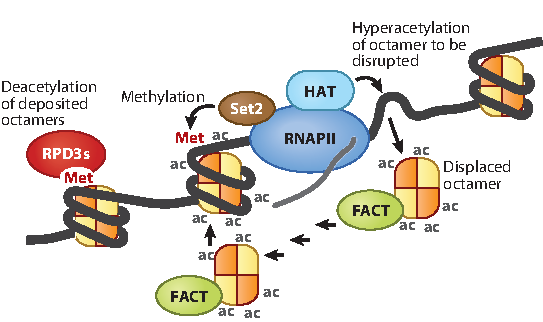
\includegraphics[width=\textwidth]{figures/introduction/nucTranscription}
\caption[Mechanism of transcription through chromatin.]{Overview of the main actors in the mechanism of transcription through chromatin.
Nucleosomes are destabilized through acetylation and chaperoned away---either partially or completely---by \gls{fact} and other complexes.
Addition of methyl groups to histone tails allows the recruitment of \gls{hdacs} and the restoration of chromatin structure.
adapted from \citep{selth:2010:transcript}. }
\label{fig:nucTranscription}

\end{figure}

The \gls{tec} can overcome this problem by enlisting the help of several histone chaperones and chromatin remodeling complexes, as well as by exploiting post translational modifications of histones (Fig: \ref{fig:nucTranscription}). 
The current model for transcription through nucleosomes posits that, depending on the intensity of transcription, histones can either be completely removed from DNA, or be partially destabilized as to allow \gls{pol2} to more easily transcribe through them \citep{kulaeva:2013:mechanism}.
The most notable actors in this phase are \gls{hats} such as Gcn5 and the \gls{fact} (\glsdesc{fact}) complex \citep[for review see:][]{reinberg:2006:de}. 
\gls{hats} are posited to travel with the polymerase, depositing an acetyl group on histone tails.
This has the consequence of destabilizing intra-nucleosome interactions, resulting in a more relaxed chromatin structure and more unstable nucleosomes.
Once histones are acetylated, \gls{fact}---also travelling with the polymerase---destabilizes the H2A-H2B dimer \footnote{
Two of the four core components of a histone. Histones are composed of two H2A-H2B dimers and one H3-H4 tetramer arranged in a symmetrical structure. 
}, removing it and facilitating transcription through the remaining incomplete nucleosome structure. 

Because of the importance of chromatin in preventing spurious initiation, the composition, modifications, and overall structure of nucleosomes must be reset after the passage of \gls{pol2}. 
Specific histone chaperones such as Spt6, together with methil-transferases and \gls{hdacs}, are involved in this process.
First, Spt6 and other histone chaperones reconstruct a complete histone in the wake of transcribing \gls{pol2}.
Subsequently, methil-transferases such as Set2 act by methilating lysine 36 on histone H3. 
Although this modification---unlike acetylation---has no structural consequences on the organization of nucleosomes, it can act as a platform for recruitment of \gls{hdacs}.
The RPD3 complex has high affinity for H3K36 methilation and is recruited immediately after the passage of \gls{pol2} in order to remove the acetyl groups from histones and thus reset the structure of chromatin.

\subsection{Transcriptional pausing} \label{pausing}
Nucleosomes do not represent the only obstacle to productive elongation.
A number of occurrences can prevent \gls{pol2} from elongating forward, such as DNA damage, misincorporation of a nucleotide, or collision with another DNA-bound protein.
While the cell has evolved complex---and often slow---mechanisms to deal with the more extreme instances \footnote{For example when DNA is damaged,the cell employs ubiquitinylation and degradation of the largest subunit of \gls{pol2} to resolve pausing.}, transcriptional pausing represents the first and common consequence to all the above-cited events. 
Because reversible pause-inducing events are relatively common during transcription---pausing has been documented in front of every nucleosome \citep{churchman:2011:nascent}---the cell evolved an all-purpose mechanism called backtracking.
The purpose of backtracking is to quickly resolve pausing before the slower, more complex systems are called into action. 

During backtracking---being unable to translocate forward---\gls{pol2} moves backwards, retracing its steps anywhere form 4-5 up to 12-15 nucleotides \citep{cheung:2011:structural}.
This backwards movement causes part of the already synthesized RNA to slide forward into a channel connected to the outside of the complex.
Presence of RNA into the channel promotes the binding of TFIIS \footnote{Also known as \emph{Dst1}} to the complex \citep{cheung:2011:structural}.
This stimulates the intrinsic endonucleolytic activity of \gls{pol2}, which results in cleavage of the extruding RNA and realignment of the 3' end of the nascent transcript with the catalytic site of the polymerase.
At this point, \gls{pol2} has effectively reset its position, having moved back and gotten rid of the extra segment of RNA. 
It can therefore restart its forward translocation and resume the normal catalytic activity.

While this mechanism is a very effective way of dealing with minor pausing events and nucleotide misincorporations, it is not enough to deal with more stubborn pausing agents.
Notably, it has been recently shown that presence of the transcription factor Reb1 on DNA is sufficient to pause the elongation of \gls{pol2} in a way that is unaffected by backtracking; ultimately resulting in the disassembly of the elongation complex and release of the transcript \cite{colin:2014:roadblock}.
 


\subsection{The CTD}
\gls{pol2} and the elongation complex are fundamental elements in coordinating many of the co-transcriptional processes that contribute to the maturation of the nascent RNA.
In order to dynamically recruit all the necessary factors and complexes in a timely fashion, the largest subunit of \gls{pol2} has evolved an unstructured C-terminal domain composed, in \cer, of 26 repeats of the heptapeptide \ctdshort{} \footnote{\ctdlong{} in expanded nomenclature}.
This cluster of repeats can be differentially phosphorylated in different phases of transcription elongation, acting as a dynamically changing interaction surface for different co-factors. 

\subsubsection{CTD phosphorylation dynamics} 
The \gls{ctd} heptapeptide contains a high number of phosphorylatable residues.
Out of the 7 amminoacids, 5 can support the addition of a phosphate group: \tyr{}, \sert{}, \thr{}, \serf{}, and \sers{}.
The combinatorial phosphorylation of \sert{} and \serf{}, however, provides the majority of the functional contribution to transcription elongation and it was recently shown that phospho-groups at these two residues are more abundant than on any of the other residues \citep{suh:2016:direct}. Unlike \sert{} and \serf{}, understanding of the consequences of \tyr{}, \thr{}, and \sers{} phosphorylation is still limited. 
Modification of \thr{} and \sers{} has specialized roles in the transcription of particular species\footnote{In vertebrates, \thr{} has been shown to be important in the processing---but not transcription---of histone genes \cite{hsin:2011:rnap}, while \sers{} was shown to recruit the \gls{ctd} phosphatase Rpap2 specifically to \gls{sns} genes \citep{egloff:2012:role}.}, while the modification of \tyr{} has no attributed roles as of yet. 
In light of this, in the following paragraphs I will focus mainly on the mechanisms and effects of \sert{} and \serf{} phosphorylation.

\begin{figure}[ht]

\centering
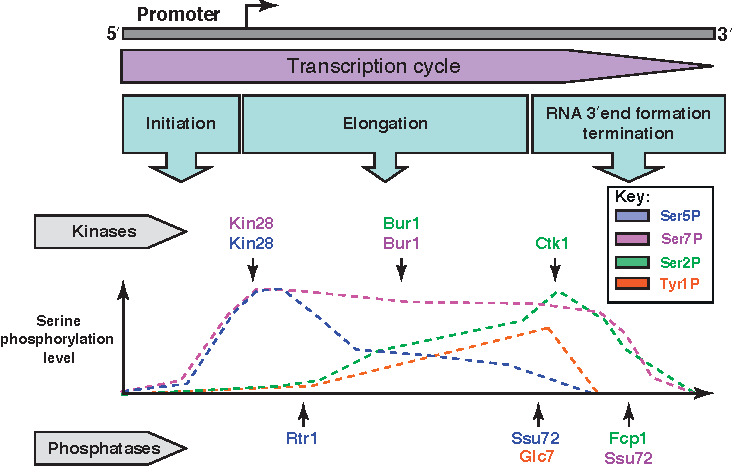
\includegraphics[width=\textwidth]{figures/introduction/ctdPhospho}
\caption[CTD phosphorylation states throughout the transcription cycle.]{
General view of \sert{}, \serf{}, and \sers{} phosphorylation along the transcription cycle,
kinases and phosphatases involved in \gls{ctd} modification are represented immediately above and below the graph.
The two main phosphorylation states, \sert{} and \serf{}, are dominant at the 3' and 5' respectively, reflecting their functional roles in the termination and early elongation phases of transcription.
\sers{} is consistently present throughtout the transcription cycle, but its functional impact in yeast remains elusive. Adapted from \citep{egloff:2012:updating}.
}
\label{fig:ctdPhospho}

\end{figure}

During the Initiation phase of transcription, the \gls{ctd} of \gls{pol2} starts off unphosphorylated (see Fig: \ref{fig:ctdPhospho}).
When the \gls{pic} is fully assembled, Kin28, a catalytic subunit of the general transcription factor TFIIH, phosphorylates the CTD heptapeptide on \serf{}.
In \cer{}, the \gls{ctd} remains mostly \serf{} phosphorylated for the first 450 nucleotides of transcription elongation \citep{mayer:2010:uniform}. 
After this point the combined action of the \serf{}-phosphatase Rtr1 \citep{mosley:2009:rtr1, hunter:2016:phosphatase} and the \sert{}-kinases Bur1 and Ctk1 \citep{qiu:2009:phosphorylation} make \sert{} the most prominent mark \footnote{
It is interesting to note that the phosphorylation state of \gls{pol2} \gls{ctd} is independent of transcript length, but exclusively depends on the amount of nucleotides from the \gls{tss}. 
This will have important implications for the termination of non-coding transcripts.}.
Despite phosphorylation of \sert{} reaching saturation about 600 nucleotides from the \gls{tss} \citep{mayer:2010:uniform}, \serf{} phosphorylation is still present on many repeats, resulting in the presence of a double phosphorylation pattern with important functional consequences (see below).
Only Towards the 3' end of the gene the action of \gls{ctd} phosphatase Ssu72 completely abrogates the \serf{}-P mark, leaving \sert{}-P as the only active mark.
Finally, additional activity of the Fcp1 phosphatase results in the removal of most phospho-marks from the \gls{ctd}, readying the polymerase for another round of transcription.

%Recent studies tried to explore the differences between distal and proximal \gls{ctd} repeats, 
\subsubsection{Functional interactions}

As I outlined above, the transcription cycle follows specific patterns of \gls{ctd} phosphorylation: unphosphorylated \gls{ctd} is recruited to promoter regions, \serf{}-P dominates during early elongation and gradually makes way for \sert{}-P, which is the dominant mark in the later stages of transcription. Each of these stages comes with the potential to interact with numerous co-factors and provides modularity to the elongation complex.

The unphosphorylated state of free-form \gls{pol2} \gls{ctd} allows the polymerase to interact with the mediator complex; an interaction that is thought to contribute to the recruitment of \gls{pol2} to active promoters. 
Once the \gls{pic} is assembled, the polymerase needs to escape the promoter and leave the \acrlong{pic} behind.
The modifications that take place at this stage, namely \serf{} phosphorylation, are thought to disrupt the interaction between \gls{pol2} and mediator---thereby allowing promoter clearance---although evidence remains inconclusive \citep{so:2007:hyperphosphorylation, davis:2002:structure}.

The presence of \serf{} mark during early elongation has two direct consequences: it stimulates capping of the nascent transcript through recruitment of the capping enzymes, and it has the potential to promote early transcription termination through the recruitment of the \gls{nns} complex.
While capping is ubiquitous and required to prevent premature degradation of the transcript, early termination is a quality control mechanism that requires (in addition to \serf{}-P) the presence of specific sequence elements on the nascent transcript and will be described in detail in a future section.

Studies in mammals have reported that the \gls{ctd} is required for splicing to occur properly, in particular heptapeptides containing both \serf{} and \sert{} phopshorylation are known to recruit several splicing factors. Recent studies in \cer{}, however, show differential phosphorylation patterns in intronless and intron-containing genes, hinting at a possible splicing role for \gls{ctd} phopshorylation in yeast \cite{milligan:2016:strandspecific}.

Towards the end of the transcription cycle, \sert{}-P becomes the most prominent mark. 
This phase sees the recruitment of a number of different actors.
Chromatin remodelers and histone modifying complexes such as Set2 and Spt6 are recruited through the \gls{ctd}, making sure that the structure of nucleosomes is maintained.

Finally, 3' end processing, termination, and export are all affected by the \gls{ctd}. binding of components of the cleavage and polyadenylation complex such as Pcf11 and Rtt103 stimulates the termination of transcription and the processing of the transcript 3' end (such as poly(A) tail addition), while recruitment of export factors such as Yra1 direct a rapid and efficient export to the cytoplasm.
 


\clearpage
	\chapter{Transcription Termination} \label{termination}
%do writing new stuff in the morning, fixing in the afternoon.
%reset in case acronyms are cited previously, this is their main paragraph and the acronym needs to be in long form.
\glsreset{cpf}
\glsreset{nns}
After its synthesis and maturation are complete, the nascent RNA molecule must be released from the DNA template, and the elongation complex must be disassembled and its components recycled.
In \cer{}, transcription termination is enacted by several widely different mechanisms.
Two predominating pathways terminate the vast majority of transcripts generated by \acrlong{pol2}: the \gls{cpf} pathway and the \gls{nns}  pathway. 
Both these mechanisms rely on short sequences on the nascent RNA---coupled with specific modifications on the \gls{ctd} of \gls{pol2}---to recruit specific factors and enact the disassembly of the elongation complex and the release of the transcript in the nucleus.

In addition to the two main pathways cited above, several non-canonical termination mechanism have been described.
these mechanisms are dedicated to the termination of specific RNA species, or can act as backups when the main pathways fail.


Finally, transcription termination is strictly intertwined with some steps of 3' end processing and maturation, strongly influencing the fate of the transcript. 
%The \gls{cpf} complex couples termination with a polyadenylation step and export competence of the RNA was shown to require this termination mechanism. 
%On the other hand, \gls{nns} is known to lead to either processing (for certain species such as \gls{sns} and \gls{snos}) or complete degradation of the transcript.



\section{The CPF-CF pathway}
The \gls{cpf} pathway was the first termination mechanism described in \cer{} because of its association with the termination of protein-coding genes\footnote{Its activity can extend to certain kinds of non-coding transcripts as well (see chapter \ref{pervasiveTranscripts} for details)}. 
\gls{cpf} termination is unique as it results in cleavage of the nascent RNA before termination occurs.
The site of cleavage is specified through sequence elements present on the nascent RNA and plays an important role in kickstarting the termination reaction.

The main actor of this termination mechanism is the \gls{cpf} complex, a large assembly of modular sub-complexes that act in concert to execute all the required steps. 
This complexity makes \gls{cpf} the most reliable, efficient, and precise termination mechanism in \cer{}.

%There exist some controversy about how \gls{cpf} termination mechanistically occurs.
%The literature proposes two models that explain termination through the \gls{cpf} pathway.
%The allosteric model argues that transcription through the cleavage site leads to conformational changes in the elongation complex, leading to destabilization of the complex and eventually termination.
%On the other hand, the torpedo model posits that after cleavage, the uncapped 5' end of the polymerase-associated transcript is attacked by exonuclease Rat1, leading to the dismantling of the complex through destabilization of the ternary complex once Rat1 catches up with the polymerase.



\subsection{Recruitment and assembly}
%TODO{figure}
Recruitment and initial assembly of the \gls{cpf} complex onto the nascent RNA is promoted by two mechanisms: interaction with specific sequences elements, and interaction with the polymerase \gls{ctd}.

A key component of the \gls{cpf} complex, Pcf11, contains a peptide sequence able to recognize the \gls{ctd}. This \gls{cid} is able to specifically recognize the \sert{}-phosphorylated version of the heptapeptide.
Given the nature of this \gls{ctd} modification---which is confined to the later stages of transcription---density of the \gls{cpf} complex around the polymerase is selectively increased where the complex is more likely to be needed for termination (i.e. at the 3' end of transcription units), facilitating the eventual binding of \gls{cpf} to the sequence elements on the nascent RNA.

Unlike in human, where the cleavage site is defined by a single highly conserved hexanucleotide sequence on the nascent RNA, Yeast \gls{cpf} complex recognizes a number of degenerate short sequences.
Two sub-complexes of \gls{cpf}, \gls{cf1a} and \gls{cf1b}, are responsible for the recognition of these sequences.
In particular, Rna15 and Hrp1 (components of \gls{cf1a} and \gls{cf1b} respectively) directly bind the nascent RNA.
Associated factors Rna14 and Pcf11 contribute to the assembly of the whole complex by interacting with \gls{pol2} and forming a scaffold that serves to tether the catalytic portion of the \gls{cpf} complex to the cleavage site.

The bulk of the catalytic activity of the \gls{cpf} complex is contained in the \gls{cpfa} sub-complex.
\gls{cpfa} directly contacts the cleavage site with its Ysh1 subunit and is responsible of the cleavage of the nascent RNA, one of the events that is thought to kickstart the termination reaction.
\gls{cpfa} also coordinates the polyadenylation reaction through the subunits Yth1 and Fip1. 
These factors recruit and tether the poly(A) polymerase Pap1 to the complex, which will begin catalyzing the addition of a poly(A) tail after the transcript has been cleaved.

Despite the wealth of knowledge available on the mechanics of \gls{cpf} recruitment and assembly, some controversy still surrounds the actual termination mechanism.
Two main models describing the termination reaction exist in the literature, the allosteric model and the torpedo model.

\subsection{The allosteric model}

After cleavage and release of the nascent RNA, the elongation complex has successfully accomplished its job in the transcriptional process and is ready to be disassembled.
The allosteric model is one of the two main mechanistic models that describes the process by which the \gls{tec} is removed from the DNA template.

The allosteric model argues that cleavage is a dispensable signal, and that termination can happen independently of this step.
It posits that after transcription of the cleavage site, \gls{pol2} loses a lot of factors that qualify the elongation complex as such.
The loss of these ``anti-terminator" factors---components of the elongation complex that would prevent termination from occurring---would trigger conformational changes, destabilize the polymerase, and allow components of the \gls{cpf} complex itself to elicit the disassembly of \gls{pol2} from the template.

Several studies support this model. 
\gls{pol2} was shown to lose a number of associated elongation factors after reaching the 3' end \citep{kim:2004:transitions}.
In addition, the component of the \gls{cpf} complex Pcf11 was shown to be able to terminate the polymerase \invitro{} by binding the nascent RNA and the \sert{}-phosphorylated moiety of \gls{pol2} \citep{zhang:2005:ctddependent}.
Ulterior support to this last study was provided by the same authors two years later, when they discovered that Pcf11 is able to perform the same feat in drosophila \citep{zhang:2006:pcf11}.
Finally, a very recent study published on Molecular Cell was able to reconstitute transcription termination in an \invitro{} system in the absence of cleavage \citep{zhang:2015:polya}.

\subsection{The torpedo model}



According to the torpedo model, cleavage represents the main termination signal for the \gls{cpf} complex, as it leaves an uncapped 5'-P on the transcript associated with the still transcribing elongation complex.
These unprotected 5' is the substrate of \FtoT{} exonucleases, a class of enzymes that are known to progressively degrade RNA polypeptides.
The \FtoT{} exonuclease Rat1 was discovered to be associated with the \gls{cpf} complex and is thought to attack the 5' moiety of the \gls{pol2}-associated transcript, starting a processivity race with \gls{pol2}.
Upon winning the race, Rat1 would destabilize the structure of the ternary complex within the polymerase, causing it to break apart and detach from the DNA template.

There are several lines of evidence that support this model for \gls{cpf} transcription termination.
Both Rat1 and its human homolog Xrn2 exhibit termination defects in model cases when mutated \citep{kim:2004:yeast, west:2004:human}.
Furthermore, Rat1 and its co-factor Rtt103 were found to be strongly associated with the 3' end of genes and in physical association with the \gls{cpf} complex \citep{kim:2004:yeast,luo:2006:role}, supporting the idea of a functional recruitment to zones of active transcription termination.
Homology studies found that homologs of Rtt103 in both humans and \cele{} have roles in transcription termination \citep{morales:2014:kub5hera, cui:2008:genes}.
Finally, recent mechanistic studies \invivo{} have demonstrated the kinetic competition between Rat1 and the elongation complex. By employing mutant polymerases that elongate faster or slower than the wild type version, the authors were able to show that slower polymerases result in earlier termination, consistent with the notion that Rat1 needs to physically catch up with the polymerase in order to elicit termination \citep{fong:2015:effects}.

At the same time, several reports argue against the torpedo model as sole effector of transcription termination.
\emph{In vitro} studies were unable to reproduce the termination effect observed \invivo{} using only Rat1  \citep{dengl:2009:torpedo}. More recent ventures re-attempted the \invitro{} approach with limited success  \citep{park:2015:unraveling}, but managed to demostrate that Rat1 is able to terminate polymerases that are destabilized by nucleotide misincorporation.
Several additional mechanistic studies showed that the exonucleolytic activity of Rat1 is unable to mediate the release of the polymerase from the template \citep{luo:2006:role, pearson:2013:dismantling}.
Moreover, termination defects caused by Rat1 mutants were not associated with stabilization of the \gls{pol2}-associated transcript, arguing against the model.
%Finally, recent genome-wide studies were unsuccessful in detecting a widespread effect of Rat1 human homolog (Xrn2) in transcription termination\citep{nojima:2015:mammalian}.


\begin{figure}[ht]

\centering
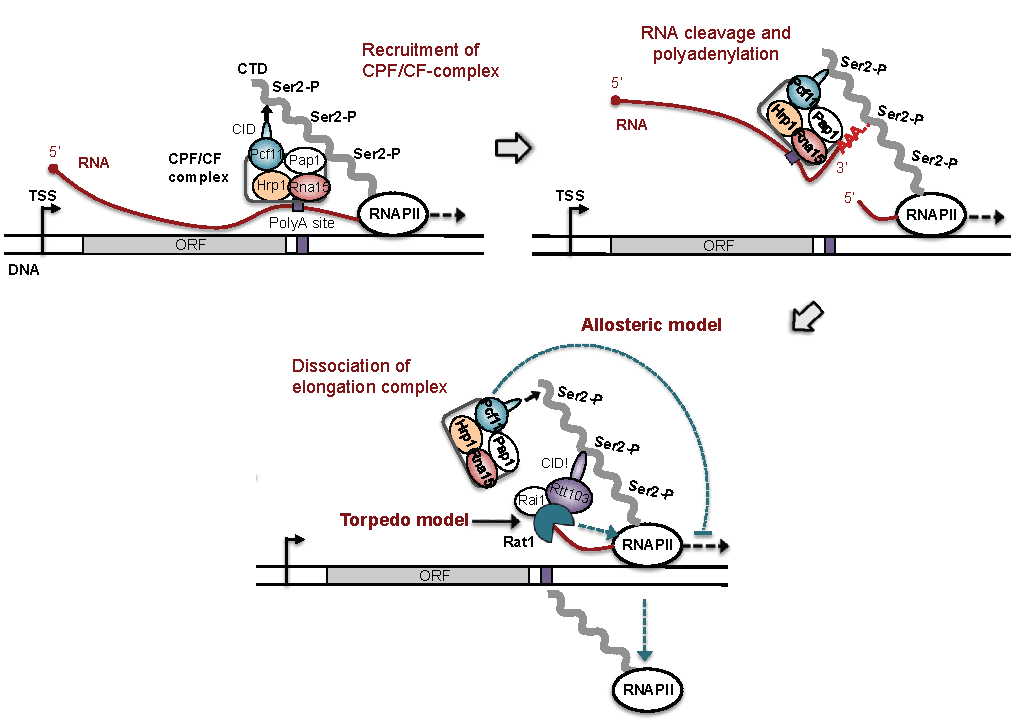
\includegraphics[width=\textwidth]{figures/introduction/cpf}
\caption[Mechanism of CPF-CF termination]{Overview of the main mechanistic step that lead to CPF-CF termination. The complex is recruited thanks to CTD phosphorylation and binding sites on the RNA. The transcript is then cleaved and the elongation complex terminated in accordance with the torpedo or allosteric model.}
\label{fig:cpfTermination}

\end{figure}

\subsection{A unified view of CPF-CF transcription termination}

As evidence for and against the two models piles up, a unified view that combines elements of both torpedo and allosteric model is taking shape.
While the effect of Rat1 on transcription termination (of at least some transcripts) is established, its role as main effector of \gls{cpf} termination has been repeatedly called into question.
Several studies have now described interdependencies between Rat1 and other subunits of the \gls{cpf} complex---notably Pcf11---and the perceived nature of Rat1 is shifting towards that of a molecular effector  that is integrated into a larger system.
The proof of principle that termination is possible without cleavage has been recently provided---albeit \invitro{} \cite{zhang:2015:polya}---and presence of Rat1 has been convincingly shown to facilitate termination \cite{fong:2015:effects}, arguing for a model that integrates these two mechanisms.

%Despite recent advances and the rise of a unified model for transcription termination, mechanistic details on the termination reaction and what prompts it are still sorely lacking.



\section{The NNS pathway}

NNS dependent transcription termination is the second of the main termination mechanisms in S.cerevisiae. 
It is essentially involved in the termination of small Nuclear RNAs (snRNAs), small Nucleolar RNAs (snoRNAs) and a number of other non-functional non-coding RNAs.
It sets itself apart from CPF-CF termination in a number of ways.
First and foremost, it relies on a completely different---and much smaller---set of proteins: the two RNA binding proteins Nrd1 and Nab3 \cite{conrad:2000:yeast}, together with the helicase Sen1. 
Because of the different molecular effectors, the termination mechanism---although still not fully elucidated---is appreciably different. 
Termination is not associated to cleavage of the nascent RNA, and release of the transcript occurs upon disassembly of the elongation complex itself \cite{steinmetz:2001:rnabinding}. 
As a consequence, the 3’ end of the terminated transcript coincides with the termination sites on DNA. 
The NNS complex also distinguishes itself because of the different fate imposed on the RNA released: instead of being exported to the cytoplasm after polyadenylation, the transcripts released are subjected to the activity of degradation enzymes (the nuclear exosome, see below) \cite{vasiljeva:2006:nrd1}. 
To this end the NNS complex recruits both the nuclear exosome and a specific set of 3' end processing factors known as TRAMP (Trf4/Air2/Mtr4p Polyadenylation), which drives polyadenylation and stimulates degradation \cite{lacava:2005:rna, vasiljeva:2006:nrd1}.

NNS termination operates mainly on non-coding RNAs and is generally restricted to the early stages of transcription elongation. 
Despite not being directly involved in the termination of protein-coding genes, it can play a role in the regulation of gene expression by acting as an attenuator \cite{arigo:2006:regulation}(i.e. terminating some transcription events, preventing them from producing functional RNAs), like in the case if IMD2 or URA2 genes \citep{jenks:2008:properties}, or otherwise terminating transcription of non-coding RNAs that might be involved in regulation \cite{thompson:2007:cytoplasmic}.



\subsection{The NNS complex}

The main molecular effectors of the NNS complex are the three protein Nab3, Nrd1, and Sen1.


\paragraph{Nab3}

This factor was originally identified as a polyadenylated RNA binding protein. 
Nab3 contains several structural domains: a conserved RNA Recognition Motif (RRM) that can contact specific sequence elements on the nascent RNA, a region necessary for the interaction with Nrd1, and an essential Glutammine/Proline region at the C-terminus.

Biochemical experiments have shown that Nab3 forms a stable heterodimer with Nrd1 and contacts the RNA as such \cite{conrad:2000:yeast}. 
In addition, the structure of the RRM has been solved, revealing the structural basis for the preference of the sequence UCUUG \cite{lunde:2011:structural}. 
Finally, its Glutammine/Proline region---despite being generally unstructured---can assemble into amyloid structures \cite{orourke:2015:amyloidlike}.


\paragraph{Nrd1}

Identified as part of the ``nuclear pre-mRNA downregulation" family of proteins, Nrd1 is the most abundant of the three members of the complex. 
Its main features consist of an RRM structure that allows it to contact the nascent RNA, a CTD interaction domain (CID) that mediates the interaction with RNAPII (see below) and a Nab3 interaction motif that allows it to form a stable heterodimer.

Nrd1's RRM was shown in vivo to contact the consensus sequence GTA[A/G] \cite{steinmetz:1998:control}. 
Recent in vitro studies, however, have shown that several other G-rich and A-rich sequences could be bound equally well \citep{bacikova:2014:structure}, although the in vivo relevance of these studies remains to be demonstrated. 

In addition to the RNA, Nrd1 can contact RNAPII through its CID \cite{kubicek:2012:serine,vasiljeva:2008:nrd1nab3sen1}. 
Although dispensable for cell viability, the CTD-CID interaction is required for efficient termination (see below).

Curiously, Nrd1 also contains a Glutammine/Proline region at the C-terminus, similarly to Nab3. 
Deletion of this region shows no growth or termination defects, but is synthetic lethal if combined with other aphenotypic mutations on Nab3 [our unpublished data]. 
The functional implications of these genetic interactions are still unknown.
 

\paragraph{Sen1}

This extremely large (253kDa) and very low abundance (125 molecules per cell) protein is the only member of the NNS complex to have enzymatic activity \cite{steinmetz:1996:repression}. 
Sen1 was characterized as a helicase of the SFI superfamily and is very closely related to Upf1, a member of the Non-sense Mediated mRNA Decay (NMD) pathway in the cytoplasm. 
Unlike its close relative, Sen1 possesses a nuclear localization signal and acts in the nucleus, where it can physically interact with the other members of the NNS complex Nrd1 and Nab3. 

Structurally, Sen1 contains a helicase domain able to hydrolize ATP and a large N terminal domain. 
The helicase domain was recently purified in E.coli and biochemically analyzed, revealing binding affinity for both DNA and RNA, but a slower translocation rate on RNA \cite{martintumasz:2015:saccharomyces}. 
Moreover, its ATPase activity was shown to be necessary for termination in vitro \cite{porrua:2013:bacteriallike}. 
The N-terminal region of Sen1 was implicated in the interaction with the RNAPII, as well as other factors such as Rnt1 and Rad2, but the implications of the latter interactions remain obscure.

\subsection{The mechanism of transcription termination}

As in the case of CPF-CF, the NNS complex is recruited to the region of termination through two distinct mechanisms that cooperate to maximize efficiency: the CTD of the polymerase \cite{vasiljeva:2008:nrd1nab3sen1} and specific sequence elements on the nascent RNA \cite{conrad:2000:yeast}. 
Within the NNS complex, Nrd1 and Nab3 are the major interactors of these elements, providing specificity and ensuring that Sen1---believed to be the molecular effector of NNS termination---is recruited only in the appropriate circumstances \cite{porrua:2013:bacteriallike}.

The CTD of RNAPII is contacted by the CID domain of Nrd1. 
This domain preferentially recognizes the Ser5-phosphorylated variant, which is the prevalent CTD phosphorylation state in the first 500-600 nucleotides of transcription. 
This preference confers to the NNS complex a high degree of specificity for terminating transcription in the early stages of elongation. 
According to the current model for NNS termination, the interaction with the CTD occurs prior to RNA binding, and facilitates recognition of sequence elements on the nascent transcript.  
Presence of Ser5-P CTD was shown to be a pre-requisite for efficient termination, as placing high efficiency NNS binding sites at the end of long transcription units---where the levels of Ser5-P would be completely supplanted by Ser2-P---does not result in termination \cite{gudipati:2008:phosphorylation}.

\begin{figure}[ht]

\centering
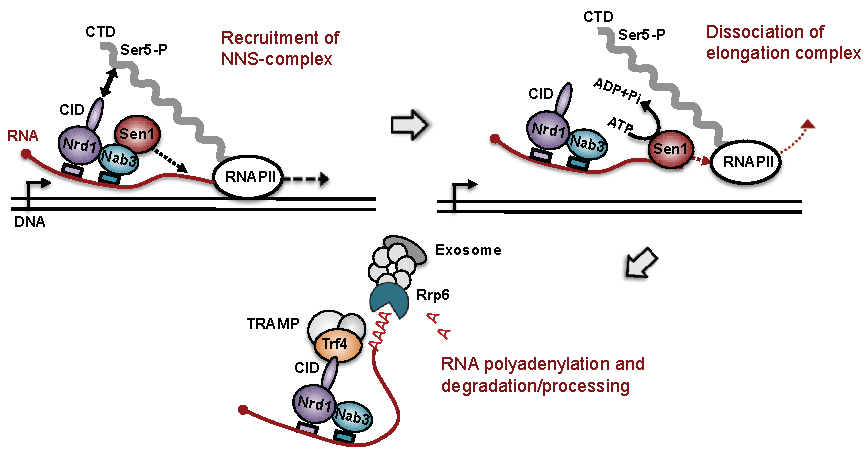
\includegraphics[width=\textwidth]{figures/introduction/nns}
\caption[Mechanism of NNS termination]{Main stages of NNS-dependent termination. the NNS complex is recruited thanks to \serf{}-phosphorylated CTD and sequence elements on the transcript. Termination is elicited by Sen1, presumably by translocating along the transcript. Finally, the exosome is recruited to the transcript and the transcript is either trimmed or completely degraded.}
\label{fig:nnsTermination}

\end{figure}

Recruitment of Nrd1 to the CTD, however necessary, is not sufficient to trigger termination. 
The Nrd1-Nab3 heterodimer must also contact the nascent RNA through the RRM domains of the two subunits.
Original studies have investigated the sequence elements that drive NNS termination, pinpointing two core consensuses: UCUU as the main binding site for Nab3, and GUA[A/G] as the main site for Nrd1 \cite{carroll:2004:identification}. 
More recent investigations redefined these consensuses and identified new sequence elements that can increase termination efficiency when in proximity of canonical binding sites. 
Use of an in vivo SELEX (Systematic Evolution of Ligands by Exponential enrichment) strategy allowed to extend the core consensus sequences for both Nrd1 and Nab3 with nucleotides that proved critical for binding (see fig ??) \cite{porrua:2012:in}. 
In addition, AU-rich sequences found downstream of Nrd1 sites were shown to play a role in increasing both termination efficiency and recruitment of Nrd1 \cite{porrua:2012:in}. Similar conclusions have been reached by in vivo crosslinking studies \cite{wlotzka:2011:nuclear}.

Despite the efforts expended in identifying sequence elements that could univocally lead to NNS termination, a lot of ambiguity remains on what constitutes an NNS terminator \invivo{}. 
While presence of Nrd1-Nab3 binding sites is required, no consistent pattern emerges in number, spacing, or quality of Nrd1/Nab3 sites at known NNS termination sites. 
Despite this, In vitro studies on model cases have identified some features of heterodimer binding. 
For example, mutation of Nab3 binding sites proved to be more deleterious to heterodimer recruitment than mutation of Nrd1 sites \cite{carroll:2007:interaction}. 
Moreover, multiple heterodimers were found to bind the same RNA sequence, possibly cooperatively  \cite{carroll:2007:interaction}. 
It remains impossible, however, to generalize these results beyond the few sequences tested. 
While the NNS complex could simply rely on a high number of low affinity sites to reach an occupancy threshold, it remains possible that several unseen elements play a role in qualifying NNS terminators, influencing the quantity and quality of Nrd1 and Nab3 binding sites necessary for an efficient termination.

When the Nrd1-Nab3 heterodimer is bound to the nascent RNA, the molecular effector of NNS termination, the helicase Sen1, is recruited to the complex. 
Studies have shown that Sen1 is strictly required to terminate transcription, but the mechanism through which this happens is not clear. 
Significant advances in the understanding of this phenomenon came from use of an in vitro transcription termination system \cite{porrua:2013:bacteriallike}. 
In this context, Sen1 alone was found to be sufficient to disassemble the elongation complex. Termination was shown to occur preferentially at sites of pausing and to require both the interaction of Sen1 with the nascent transcript and ATPase activity. 
It is unclear whether ATP-dependent translocation of Sen1 on the nascent RNA is required for termination. However, results from an in vivo study suggest the existence of a kinetic competition between transcription elongation and Sen1 translocation on the RNA. 
The authors investigated the effect of the speed of transcription on NNS termination, showing that faster transcription results in longer NNS-terminated transcripts, while slower transcription produces shorter transcripts and is able to suppress mutations on Sen1 \cite{hazelbaker:2013:kinetic}. 
Taken together, these results support a model where, akin to the bacterial termination factor Rho, Sen1 would contact the nascent transcript and translocate in a 5’ to 3’ direction, eliciting termination upon catching up with the polymerase.

\subsection{Processing of products of the NNS pathway}

The process of NNS termination is strictly connected with 3' end processing or degradation mediated by the nuclear exosome, a multiprotein complex endowed with exonuclease activity \cite{vasiljeva:2006:nrd1}. 
The exosome plays a major role in nuclear RNA quality control, degrading aberrant transcripts, a number of non-functional non-coding RNAs, and trimming the precursors of functional small non-coding RNAs such as sn/snoRNA \cite[for review see][]{kilchert:2016:regulation}. 
The exosome is composed of six non-catalytic subunits arranged in a ring-like structure, together with three cap subunits that can bind RNA (see figure X). 
The catalytic activity of this complex is dependent on two active 3' to 5' exonuclease, Dis3 and Rrp6. 
Dis3 associates with the ring on the opposite side of the three cap subunits, and degrades RNAs that are threaded through the cap proteins and into the ring \cite{makino:2015:rna}. 
The exosome is present throughout the nucleus and in the cytoplasm. 
However, only the nuclear version can associate with the other exonuclease, Rrp6, whose activity is known to regulate the levels of many NNS targets.

Recruitment of the exosome to NNS targets takes place via one of the exosome’s co-factors: the TRAMP complex. 
TRAMP (for Trf4/Air2/Mtr4p Polyadenylation) is a nuclear complex composed of the poly(A) polymerase Trf4, the RNA-binding protein Air2 and the helicase Mtr4. 
Trf4 is the core subunit of the complex, to which both Air2 and Mtr4 bind independently. 
It possesses poly(A) polymerase activity, but unlike Pap1---the canonical poly(A) polymerase associated with the CPF-CF complex---it can only add tails in a distributive manner. 
Trf4 is also the factor responsible for the coordination between the NNS complex and the nuclear exosome. 
A recent study showed that Trf4 contacts Nrd1 through a small motif called Nrd1 Interaction Motif (NIM) . 
The NIM on Trf4 mimicks Ser5-P CTD and can therefore compete with the CTD of RNAPII for the interaction with the CID (CTD interaction domain) on Nrd1. 
The interaction of Nrd1’s CID with the CTD and Trf4 are mutually exclusive, and Trf4 was shown to have much higher affinity for the CID. 
These findings have suggested a model whereby TRAMP is recruited to the RNA when the CID of Nrd1 is freed from the CTD of the polymerase \cite{tudek:2014:molecular}. 
This effectively allows the coordination of events going from termination to the handover of the transcript to TRAMP and the exosome.

As a co-factor of the exosome, TRAMP is able to both recruit and stimulate its activity. 
Addition of a poly(A) tail to the terminated transcript is thought to provide an unstructured platform that can be easily be threaded through the non-catalytic subunits of the exosome. 
However, TRAMP has been known to stimulate exosome activity even indipendently of poly(A) polymerase activity \cite{tudek:2014:molecular}. 

By virtue of the tight connection between NNS and TRAMP, NNS-terminated transcripts are usually subject to rapid degradation. SnoRNAs and snRNAs constitute notable exceptions, in that they are heavily structured functional non-coding transcripts that are recruited to the exosome, but undergo only trimming of their 3’ ends instead of complete degradation. This is thought to occur thanks to the presence of secondary structure and additional proteins binding the RNA, preventing the transcript from being entirely threaded through the exosome \cite{mitchell:1997:exosome}.


\section{Non-canonical termination pathways}

CPF-CF- and NNS-dependent termination seemingly account for the vast majority of RNAPII transcription termination events in the cell.
Several additional mechanisms, however, can terminate transcription in S.cerevisiae. 
These non-canonical termination pathways are generally thought to act as a fail-safe pathway in restricting readthrough transcription \cite{colin:2014:roadblock,ghazal:2005:genomewide}.


\subsection{Rnt1-dependent termination}

The yeast Rnase III homologue Rnt1 is an enzyme that binds and cleaves double-stranded RNA stem-loops at a defined recognition site. 
Rnt1’s known function in the cell is that of cleaving polycistronic rRNAs and snoRNAs transcripts, promoting their subsequent trimming and processing by the exosome \cite{ghazal:2005:genomewide}. 
Recently, Rnt1 binding sites have been identified downstream of a number of genes and its cleavage activity has been implicated in transcription termination.

Studies on the model gene NPL3 have shown that deletion of Rnt1 leads to transcriptional readthrough and can even mediate the production of dicistronic transcripts \cite{ghazal:2009:yeast}. 
Rat1, the mediator of the CPF-CF termination according to the torpedo model, was found to be also required for proper termination by Rnt1. 
This led to a model where Rnt1 cleaves a stem-loop that forms downstream of the CPF-CF cleavage site, generating a non-polyadenylated transcript, and leaving an uncapped 5’ on the nascent transcript. 
This free 5’-OH is a substrate for exonuclease Rat1, and transcription termination is thought to occur with a mechanism akin to the CPF-CF torpedo model, with Rnt1 as the cleaving agent instead of the CPF complex  \cite{ghazal:2009:yeast, rondo:2009:failsafe}.

The termination mechanism is usually very intimately connected with 3’ end processing and with the fate of the transcripts it produces. The case of Rnt1-dependent termination, however, is peculiar in this respect.
Use of in vivo reporter systems showed that, in the absence of a polyadenylation site, Rnt1-dependent transcripts are unstable and supposedly targeted by TRAMP and the exosome \cite{ghazal:2009:yeast}. 
However, addition of a cryptic polyadenylation site close to the Rnt1 binding site in the same system results in increased transcript stability that is Pap1-dependent. 
This suggests that depending on its environment, Rnt1 can either stimulate the usage of a nearby Polyadenylation site or produce transcripts that are targeted for degradation \cite{rondo:2009:failsafe}.

\subsection{Road-block termination} \label{roadblockIntro}
  
Road-block termination represents another non-canonical mechanism that can mediate transcription termination. 
Road-block was first observed as a termination mechanism for RNAPI, where  a DNA binding factor acts as a physical obstacle for the polymerase. 
The polymerase is thought to stall at the DNA binding site and eventually dissociate from the template through unclear mechanisms \cite{lang:1994:model, lang:1993:reb1}. 

When the mechanism was first described, in vitro work had shown that transcription factor Reb1 was able to pause all three yeast RNA polymerases \cite{lang:1994:model}. 
Later studies from the same authors confirmed that the DNA binding site for Reb1 was coincident with sites of RNAPI transcription termination in vivo \cite{reeder:1999:saccharomyces}. 
Combination of these experiences led to a model where Reb1 is binding DNA and terminating RNA polymerase I at specific rDNA loci. 
It was only in 2012 that a Reb1 paralogue---Nsi1, who binds the same consensus sequence as Reb1---was implicated as the true in vivo effector of RNAPI termination, while Reb1 was proven to not have a role \cite{reiter:2012:reb1homologue}. 

I have participated to a study of the laboratory showing that Reb1 is the effector of roadblock transcription termination for RNA polymerase II in vivo. 
This study will be described in the results section.

\clearpage
	\chapter{The transcriptional Landscape of \cer{}}
The rise of microarrays and next generation sequencing techniques has made the exploration of the transcriptome possible. 
Early application of tiling arrays to the transcriptome of S.cerevisiae showed that, in addition to protein coding genes and a multitude of functional non-coding RNAs, the genome is pervasively transcribed and RNA molecules can arise from many unannotated regions \cite{xu:2009:bidirectional, neil:2009:widespread,david:2006:highresolution}. 
There are multiple possible reasons for this phenomenon. 
The genome might provide an inherently low barrier to transcription initiation. 
Additionally, studies have shown that yeast promoters, despite showing directionality, can fire bidirectionally and give rise to non-functional RNAs \cite{xu:2009:bidirectional, neil:2009:widespread}. 
Promoter bidirectionality, and the general propensity of transcription to initiate spuriously, is at the origins of the widespread occurrence of transcription, which is usually referred to as pervasive transcription and contributes to the generation of large quantities of non-coding (mostly non-functional) RNAs. 

\section{Control of pervasive transcription}

Pervasive transcription represents a non-negligible fraction of all RNAPII transcription. 
Therefore, it has the potential to interfere with other physiological events and needs to be carefully regulated. 
Control of pervasive transcription occurs on two levels: First, RNAPII that initiates spuriously need to be rapidly terminated, in order to avoid interference with other processes on DNA; second, the resulting transcripts need to be efficiently degraded, to prevent accumulation of toxic species. 

The NNS complex is the main termination pathway involved in control of pervasive transcription \cite{arigo:2006:regulation, thiebaut:2006:transcription}. 
Binding sites for Nrd1 and Nab3 are frequently enriched in areas where pervasive transcription occurs, such as antisense to coding RNAs and in intergenic regions \cite{thiebaut:2006:transcription}. 
Acting early in the transcription cycle, NNS is an effective tool to block such transcription events before they can do damage. 
Despite the major role of NNS, CPF-CF, as well as some non-canonical termination pathways, have been implicated in termination of pervasive transcription \cite{marquardt:2011:distinct, vandijk:2011:xuts,colin:2014:roadblock}.

Once termination has occurred, transcripts are released into the nucleus. 
These RNA species do not possess coding potential and might be deleterious to the cell if accumulated in sufficient quantities. 
In order to prevent such accumulation, the cell evolved RNA quality control systems that can degrade spurious and aberrant transcripts. 
These decay pathways can be directly connected to termination and 3’ processing, as in the case of NNS and the TRAMP-Exosome \cite{thiebaut:2006:transcription}, or recognize specific features that mark non-functional transcripts, such as poor coding potential.

\section{Classes of pervasive transcript} \label{pervasiveTranscripts}

Because of their rapid turnover, the majority of pervasive transcripts are difficult to detect in wild type cells. 
Several studies found that deletion of certain elements of RNA quality control would affect the stability of only a subset of pervasive transcripts, making them appear in transcriptome analyses \cite{wyers:2005:cryptic, vandijk:2011:xuts}. 
Over time, it became obvious that several classes exist, each responding differently to inactivation of specific quality control pathways. 
The following classes, therefore, represent sets of transcripts sharing one or more features that make them more susceptible to specific branches of quality control.

\begin{figure}[ht]

\centering
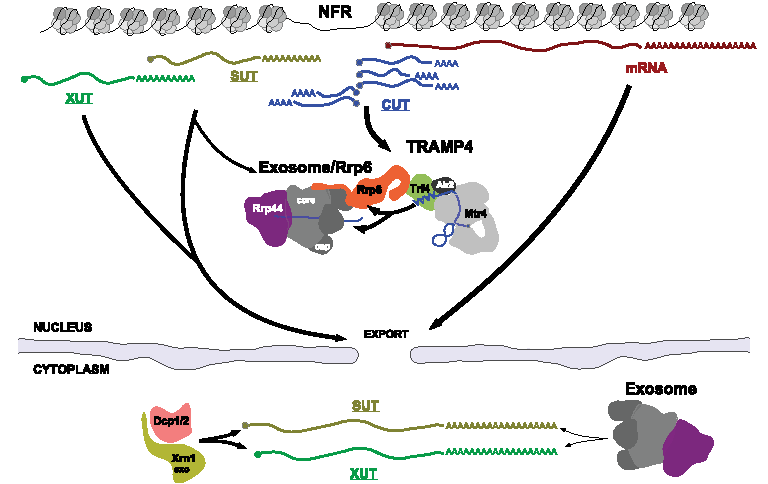
\includegraphics[width=\textwidth]{figures/introduction/pervasiveTr}
\caption[Classes of transcripts and their fates.]{The cellular fate of pervasive transcripts. Different classes of non-coding RNAs are represented at the top. Black arrows indicate the fate of the transcript after transcription, either immediate degradation via the exosome/\gls{tramp} quality control pathway, or export to the cytoplasm. Here, cytoplasmic quality control is shown.}
\label{fig:pervasiveTranscripts}

\end{figure}


\paragraph{CUTs}

The first—and most abundant—class of pervasive transcripts to be described, Cryptic Unstable Transcripts (CUTs) were identified in a strain missing the exosome co-factor Rrp6 \cite{wyers:2005:cryptic}. 
CUTs are short transcripts (400-800 bp) originating from intergenic regions and bidirectional promoters.
They can often be detected in the antisense direction to protein coding genes and their transcription can sometimes contribute to gene regulation \cite{arigo:2006:termination}. 

CUTs are terminated by the NNS pathway \cite{arigo:2006:regulation}. 
This greatly facilitates their turnover, which occurs exclusively in the nucleus. 
After transcription termination has occurred, CUTs are contacted by TRAMP and handed over to the nuclear exosome, resulting in their rapid degradation \cite{thiebaut:2006:transcription}.

\paragraph{SUTs}

Unlike CUTs, Stable Untranslated Transcripts (SUTs) are detectable in wild type cells \cite{david:2006:highresolution}. 
This difference is due to the termination mechanism that characterizes these transcripts. While CUTs are terminated early by the NNS pathway, SUTs are longer and terminate through the CPF-CF pathway \cite{marquardt:2011:distinct}. 
This difference in termination implies that SUTs can more easily escape the nucleus and be exported into the cytoplasm. 
It should be noted that a large portion of SUTs is partially affected by exosome mutations, suggesting that multiple termination mechanisms might contribute to the generation of these transcripts. 

Despite being exported to the cytoplasm, SUTs have poor coding potential and are targeted by specific quality control pathways in this compartment (see below) \cite{malabat:2015:quality}.

\paragraph{XUTs}

Very close to SUTs, Xrn1-dependent Unstable Transcripts (XUTs) have essentially the same characteristics.
They are terminated by the CPF-CF pathway and rapidly exported to the cytoplasm \cite{vandijk:2011:xuts}. 
However, while the turnover rate of SUTs is sufficiently slow to allow their detection in wild type cells, XUTs are more susceptible to cytoplasmic decay pathways, and therefore require deletion of Xrn1—the main molecular effector of cytoplasmic RNA degradation—to become visible in transcriptome analyses \cite{vandijk:2011:xuts},=.


\paragraph{NUTs}

Largely overlapping with CUTs, Nrd1-dependent Unterminated Transcripts (NUTs) are defined as transcripts that gain stability when NNS termination is impaired \cite{schulz:2013:transcriptome}. 
Normally, these transcripts are rapidly degraded by the nuclear exosome. 
However, when NNS termination is impaired, they gain in length and stability, becoming detectable.

\paragraph{RUTs}

Only recently identified as a new class of pervasive transcripts, Reb1-dependent Unstable Transcripts (RUTs) are transcripts subjected to road-block termination by the transcription factor Reb1 and subsequently degraded by the nuclear exosome \cite{colin:2014:roadblock}.

\section{Quality control pathways}

RNA quality control eliminates aberrant and pervasive transcripts through degradation. 
Several multisubunit complexes located throughout the cell carry out this function through use of endo- and exo-nuclease activities. 
Targeting of transcripts to these complexes (i.e. marking for degradation) can occur through several means: it can be directly connected to the termination mechanism used to release the transcript (as in the case of NNS termination), or it can depend on certain features of the RNA, such as presence of a premature stop codon.

The exosome is known to act in both the nucleus and the cytoplasm. 
Its catalytic activity depends on the subunit Dis3, which possesses 3' to 5' exonuclease and endonuclease activity. In the nucleus, the exosome is associated with two specific co-factors: a second 3' to 5' exonuclease called Rrp6, and a polyadenylation complex called TRAMP \cite{lacava:2005:rna}. 
While Rrp6 significantly contributes to RNA degradation through its exonuclease activity, TRAMP stimulates the activity of the exosome through addition of short poly(A) tails and other, less clear means \cite{haracska:2005:trf4,jia:2012:rna}. 
This ensemble of factors makes the exosome the foremost quality control agent in the nucleus. 
In the cytoplasm, the exosome is not found in complex with Rrp6 or TRAMP and has only a minor role in RNA degradation \cite[for review see][]{tudek:2015:noncoding}.

In the cytoplasm, RNA degradation is mainly enforced by the 5' to 3' exonuclease Xrn1. 
Several decay pathways can lead to degradation by Xrn1 (and to some extent the cytoplasmic exosome): Non-sense Mediated mRNA Decay (NMD), triggered by the presence of a premature stop codon; No-Go Decay (NGD), triggered by lack of a translation start codon; and No-Stop Decay (NSD), caused by lack of a stop codon.
These pathways target transcripts that do not possess the typical features of mRNAs, stopping potentially toxic elements from being translated \cite[for review see][]{houseley:2009:many}. 
Xrn1 is known to target pervasive transcripts with poor coding potential, such as SUTs and XUTs, providing a backup system that can deal with those RNAs that manage to escape the nuclear quality control \cite{malabat:2015:quality}.

\section{Function of pervasive transcripts}

The question of whether pervasive transcripts in yeast possess any functional activity remains unclear.
While the act of pervasive transcription has been associated with regulatory events on multiple occasions, very little is known about the function of the transcripts themselves. 

For instance, SER3 expression is known to be regulated by the upstream transcription unit SRG1—producing a non-coding RNA—through a mechanism of transcriptional interference \cite{martens:2004:intergenic}. 
This phenomenon occurs when an elongating polymerase invades a promoter, thereby reducing the efficiency of transcription initation. Similarly, the PHO84 gene seems to be regulated by an antisense transcript that runs along the whole gene, reaching the promoter and downregulating expression \cite{castelnuovo:2013:bimodal}. 
In both these cases, repression is mediated by a modification of the chromatin state of the promoter, which prevents assembly of the Pre-Initiation Complex. Stabilization of the transcript, however, did not in any way affect the repression.

Other regulation mechanisms involve NNS termination and a conditional generation of CUTs. Several nucleotide biosynthesis genes (URA2, URA8, IMD2 among others) can initiate transcription from two regions separated by an NNS terminator sequence \cite{jenks:2008:properties, thiebaut:2008:futile}. 
Only transcription from the downstream TSS results in productive elongation, while transcription starting from the upstream TSS results in early termination and degradation of the transcript. 
It has been shown that nucleotide availability modulates TSS selection, and said genes are properly expressed only when specific nucleotide concentrations are low.


\clearpage




	\boldchapter{General regulatory factors}
General Regulatory Factors (GRF) are a subset of abundant, widespread, and multi-functional DNA-binding proteins involved in several aspects of chromosomal function. 
In addition to their role as transcriptional activators, GRF are involved in transcriptional silencing, telomere maintenance, and centromere function.

The proteins defined as GRF are, among others, Rap1, Reb1, Abf1 and Cbf1 \cite{diffley:1992:global}. 
GRFs are a functionally and structurally heterogeneous group of proteins. 
However, they have the capability of activating transcription through specific binding in promoter regions and modification of the chromatin structure. 
Through this mechanism, GRF are known to regulate a substantial number of genes.

In this section, I will describe in brief the specific roles of each GRF and subsequently focus on their transcriptional activity.

\begin{figure}[ht]

\centering
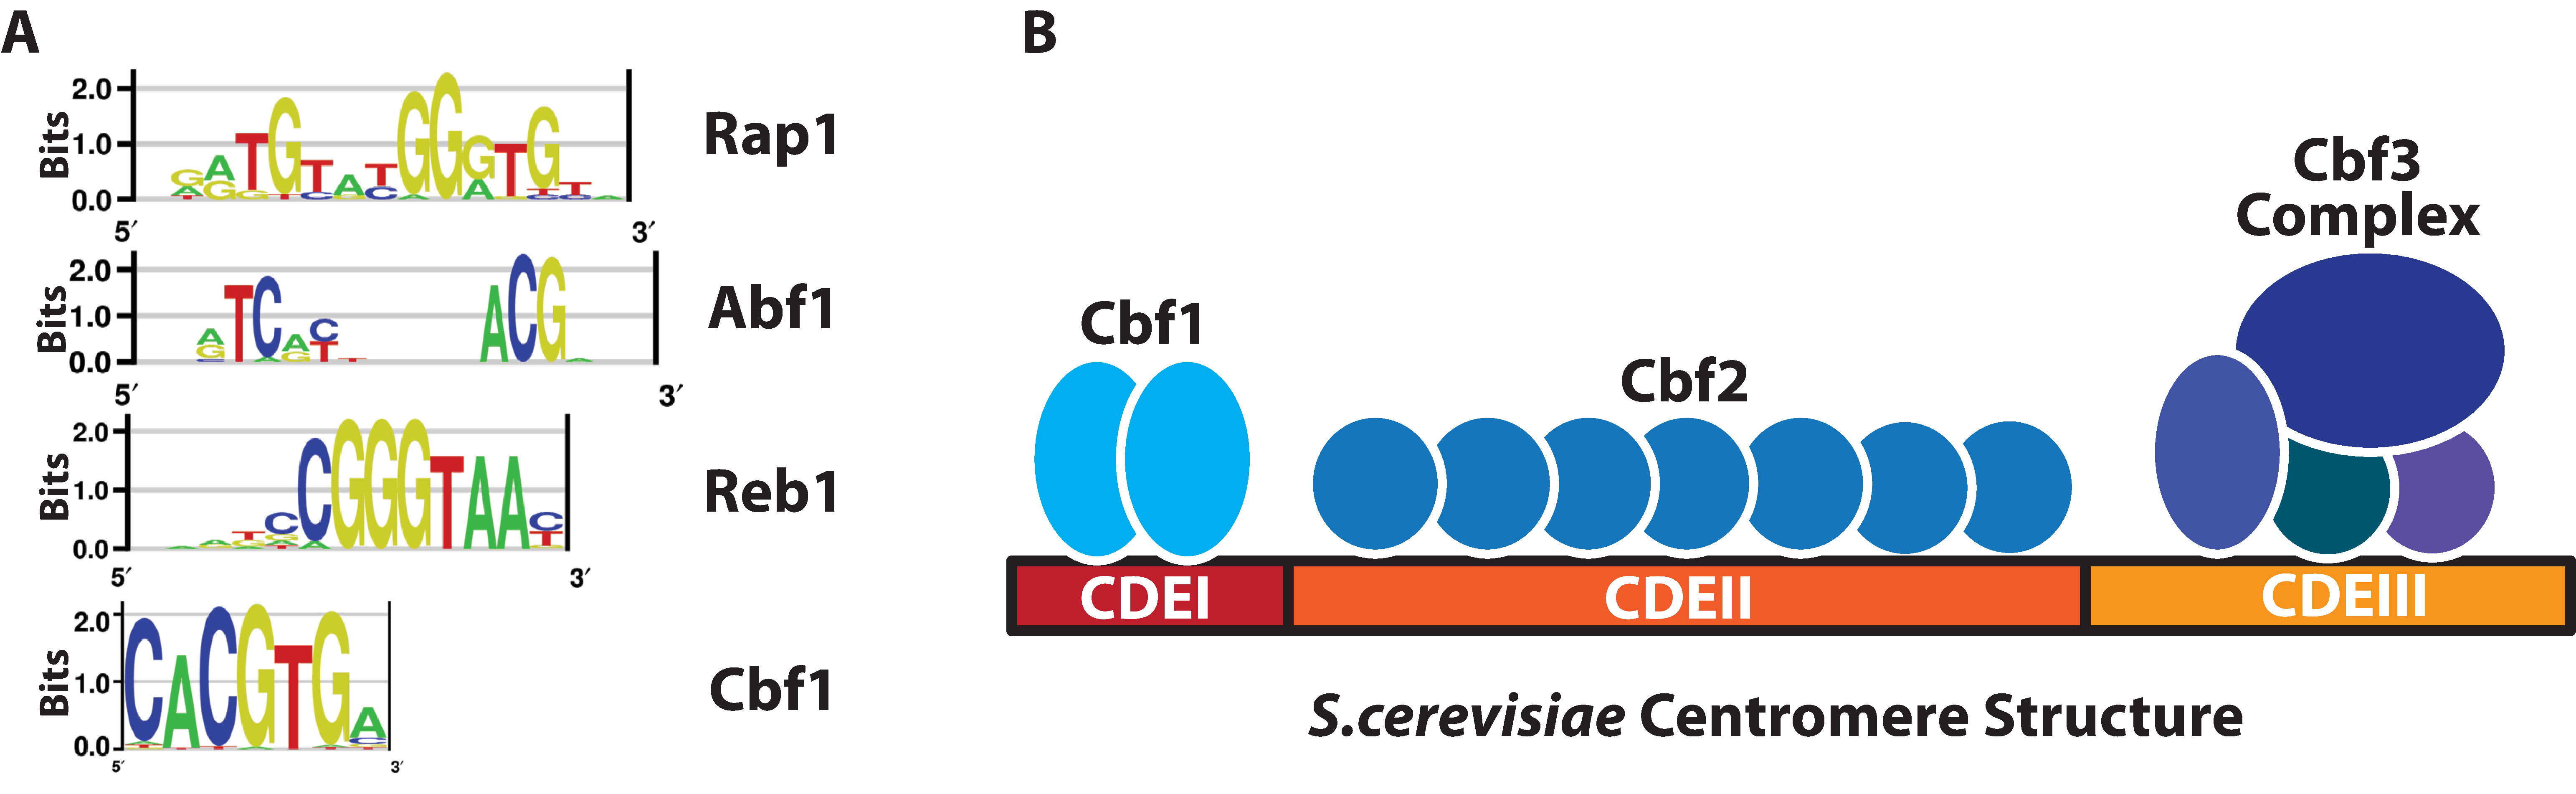
\includegraphics[width=\textwidth]{figures/introduction/grfCentromere}
\caption[GRFs binding sites and \cer{} centromere structure]{\textbf{A:} Sequence logos representing the main binding sites for the four GRFs Rap1, Abf1, Reb1, and Cbf1. \textbf{B:} structure of the centromere in \cer{} and its main interactors, A Cbf1 dimer is stably bound to CDEI.}
\label{fig:grfCentromere}

\end{figure}

\section{Rap1}

The essential transcription factor Rap1 is probably the best characterized GRF and it has a multitude of functions. 
Rap1 has a strong preference for the specific DNA element shown in figure \ref{fig:grfCentromere}A. This binding is mediated by two large DNA binding domains very similar to those of the human oncogene Myb \cite{rhee:2011:comprehensive}. 

Rap1 is the main transcriptional activator of ribosomal protein (RP) genes, controlling the expression of about 90\% of these species \cite{moehle:1991:association}. 
This regulation is enacted through multiple pathways.
First, Rap1 recruits a number of ancillary transcription factors: Fhl1, Ifh1, Sfp1, and Hmo1. Together they modify the structure of chromatin and stimulate transcription \cite{reja:2015:molecular}. 
Second, Rap1 is able to independently recruit TFIIA and TFIID to the promoter of RP genes, accelerating the rate of PIC formation at these loci \cite{papai:2010:tfiia}.


In addition to its activator capabilities, Rap1 works as an active silencer of transcription. 
During vegetative growth, the mating type loci of S.cerevisie are transcriptionally inactive. 
Their silencing is mediated by binding of Rap1, Orc1, and another GRF, Abf1. 
These proteins are able to recruit Sir1, Sir2, Sir3, and Sir4, which mediate the spread of heterocromatin over the HML and HMR loci, preventing transcription initiation \cite{kurtz:1991:rap1}. 
The transcriptional repressor activity of Rap1 has also been reported for RP genes under conditions of nutrient starvation, but in these conditions the silencing mechanism remains unclear \cite{reja:2015:molecular}. 


Lastly Rap1 has been implicated in the maintenance of telomeres \cite{lustig:1990:involvement}. 
In this context, Rap1 is part of a complex named Telosome together with Rif1 and Rif2. 
The telosome forms a protective cap around telomere sequences and is required for different aspects of telomere homeostasis such as telomere length regulation, inhibition of end resection, protection from fusion and inhibition of untimely activation of the DNA damage checkpoint \cite[for review see][]{wellinger:2012:everything}. 
Recent genome-wide studies identified Rap1 binding sites both at telomeres and RP genes, showing that these two classes of binding sites are distinct \cite{rhee:2011:comprehensive}. 
Somewhat consistent with this notion, another study showed how Rap1 possesses two binding modes. 
According to the authors, Rap1 can either bind a single site with high efficiency making use of both its Myb-like DNA binding domains, or it can bind more degenerate sequences with lower affinity using only one domain, but forming higher stoichiometry complexes \cite{feldmann:2014:dnabinding}. 
However, whether these two binding modes have functional consequences is unknown.

Rap1, together with other GRF such as Reb1 and Abf1, has been shown to have a role as as insulator (i.e. preventing the spread of heterochromatic silencing), and is thought to act in this capacity at the mating type loci \cite{fourel:2002:general}.


\section{Abf1}

Both Structurally and functionally close to Rap1, Abf1 is another essential factor implicated in numerous processes. 
Abf1 binds the split DNA site shown in figure \ref{fig:grfCentromere}A, which is known to regulate hundreds of promoters. 

While the vast majority of RP genes are regulated by Rap1, a cohort representing 10\% of the total is under the control of Abf1 \cite{dellaseta:1990:abf1}. 
A recent study investigated the mechanism of Abf1-dependent RP gene regulation, showing that Abf1 is found in association with Fhl1 and Ifh1, but has a lower occupancy on the promoter relative to Rap1 \cite{fermi:2016:multiple}. 
Abf1-dependent regulation of RP genes seems to possess distinct features from the canonical Rap1 regulation. 
Under nutrient starvation, Abf1 was observed to be more stably associated with the promoter and this resulted in a severe downregulation of gene expression. 
The authors speculated that stable association of Abf1 with DNA could mediate transcriptional silencing, while a more dynamic interaction could mediate activation \cite{fermi:2016:promoter}.

Akin to Rap1, Abf1 is known to act in silencing at the mating type loci, as well as an insulator in sub-telomeric regions \cite{mak:2009:dynamic}. 

Abf1 is present in a number of autonomous replicating sequences (hence the name ARS Binding Factor 1). 
These regions of the genome are essential to the process of DNA replication and act as its starting points.
The C-terminal region of Abf1 was found to enhance replicative activity independently of the transcription activation domain \cite{wiltshire:1997:abf1p}. 
In addition, replication factors have been shown to increase Abf1 DNA-binding activity \cite{feng:1998:saccharomyces}. 
Despite these data, however, Abf1’s mechanism of action at replication origins has never been fully elucidated.

Lastly, Abf1 is implicated in the activity of the global genome nucleotide excision repair mechanism (GG-NER). 
Abf1 was shown to form a stable complex with Rad7 and Rad16, two essential protein for GG-NER activity  \cite{reed:1999:yeast}. 
Additionally, impairing Abf1 DNA binding results in UV-sensitive yeast. 
The Rad7-Rad16-Abf1 complex is known to generate superhelical torsion in DNA \cite{yu:2004:yeast}, and Abf1 is thought to provide specificity to the complex through its DNA binding activity \cite{Yu:2009:abf1binding}.

\section{Reb1}

Reb1 was first identified as an rDNA enhancer binding protein, where it acts in stimulating transcription of ribosomal DNA \cite{planta:1995:global}. 
Reb1 tightly binds the consensus reported in figure \ref{fig:grfCentromere}A with a bipartite myb-like DNA binding domain.
Functionally, it acts to promote transcription of about 600 genes and it was implicated as an insulator in sub-telomeric regions. 
The homologue of Reb1 in S.pombe has been extensively studied as a DNA replication termination factor, as it is able to stall replication forks \cite{sa:2004:transcription}. The implication in this process in S.cerevisiae, however, is still unproven.


Reb1 was mistakenly believed to be the effector of RNAPI transcription termination \cite{lang:1995:transcription}. 
This notion, however, was dispelled when it was shown that Nsi1, a related protein that binds the same consensus on DNA, was the true molecular effector of RNAPI termination \cite{reiter:2012:reb1homologue}. 
Interestingly, Reb1 is now implicated in the termination of RNAPII through the same road-block mechanism with which it was thought to terminate RNAPI \cite{colin:2014:roadblock}.


\section{Cbf1}

Cbf1 is the only GRF thus far to not possess a myb-like DNA binding domain. Instead, it is a member of the helix-loop-helix family of DNA binding factors and specifically binds the consensus represented in figure \ref{fig:grfCentromere}A. 
Cbf1 is mostly known for its activity as a structural element in centromeres, but can stimulate transcription of a limited number of genes \cite{mellor:1990:cpf1}.


In S.cerevisiae, centromeres are short (120 nucleotides) DNA sequences coated with proteins that mediate assembly of the kinetochore and proper chromosome segregation during mitosis (Fig. \ref{fig:grfCentromere}B). 
Structurally, the centromere sequence is divided into three Centromere DNA Elements (CDE): CDEI, CDEII, and CDEIII. Cbf1 is the main binder of CDEI, a region of the centromere known to be important, but not essential for chromosome segregation \cite{niedenthal:1993:cpf1}. 

\begin{table}
\begin{tabular}[c]{cccp{4.9cm}}
\hline 
GRF & DNA-binding & \makecell{Chromatin\\Remodeling}  & Functions  \\
\hline 
Rap1 & bipartite Myb-like & multiple \cite{reja:2015:molecular} & RP genes activation, silencing of mating type loci, telomere maintenance \vspace{2mm} \\ 
Abf1 & Myb-like & RSC & RP genes activation, silencing of mating type loci, insulator, stimulator of DNA replication \vspace{2mm} \\
Reb1 & bipartite Myb-like & RSC & terminator of RNAPII, insulator \vspace{2mm} \\ 
Cbf1 & Helix-turn-helix & unknown & part of centromeres, transcriptional activator \\ 
\hline 

\end{tabular} 
\caption[characteristics of GRFs]{summary of GRF functions, binding sites and associated chromatin remodeling system.}
\label{tab:grfs}
\end{table}

Additionally, Cbf1 is known to form a complex with transcription factors Met4 and Met28. 
Through this complex, Cbf1 is able to target Met4 to genes involved in Sulphur metabolism \cite{oconnell:1995:role}. 
In addition to bringing Met4 to the promoter of MET genes, Cbf1 is also known to modify the structure of chromatin at MET and other gene loci through a still unknown mechanism.


\section{Chromatin Remodeling} 

A common feature of GRFs is the capability of altering the local chromatin structure in the vicinity of their binding sites. This mechanism is used to clear nucleosomes from promoters and thus stimulate transcription. 
As a general rule, GRFs are considered “obbligate synergizers”: they can weakly stimulate transcription on their own, but achieve a much greater effect when another weak activator binds the same promoter. 
The chromatin remodeling activity of GRFs is therefore thought to act as a force multiplier, allowing normally weakly binding transcriptional activators, who would not be able to bind a more chromatinized template, to be stably bound on DNA \cite{chasman:1990:yeast,bussemaker:2001:regulatory,pilpel:2001:identifying}.


Although all GRF described possess some level of chromatin remodeling activity, it is unclear whether this stems from use of a common system or multiple independent pathways. 
Studies implicated Reb1 and Abf1 in connection with the RSC complex \cite{hartley:2009:mechanisms}. 
To prove this point, the authors depleted Abf1 and Reb1, which resulted in a shrinkage of several NFRs.
Subsequent depletion of the catalytic subunit of the RSC complex, Sth1, showed that NFRs regulated by Reb1 and Abf1 are also regulated by RSC. 
In addition, the authors inserted a Reb1 site within an ORF and observed that an NFR could form depending on the presence of both Reb1 and of Sth1. 
These findings were confirmed by more recent investigations \cite{kubik:2015:nucleosome}, which found a large overlap between promoters regulated by Reb1 and Abf1 and promoters regulated by RSC. 
The same study, however, discovered a number of promoters where NFRs are generated in a Reb1- and Abf1-dependent manner, but independently of RSC, arguing for a more complex regulation mechanism. 



\subsection{Genome-Wide Effect on Chromatin Structure}

The stereotypical view of eukaryotic promoters is characterized by well-positioned +1 and -1 nucleosomes surrounding a 150+ stretch of poorly chromatinized DNA. 
This notion was challenged by a recent study that showed the existence of nucleosomal particles inside a large number of promoter NFRs \cite{kubik:2015:nucleosome}. 
These fragile nucleosomes (FN) are particularly sensitive to the amount of micrococcal nuclease (MNase) used to reveal nucleosome positioning in a genome-wide manner, and therefore went undetected until now. 
Analysis of the distribution of GRF binding sites inside promoters showed that fragile nucleosomes are significantly associated with GRF binding. 
Additionally, the GRF-associated chromatin remodeling complex RSC was implicated in the process, and insertion of GRF binding sites in previously unaffected promoters was shown to induce fragile nucleosome formation. 
For Reb1 and Abf1, the GRF binding site seems to coincide with the position of the fragile nucleosome, suggesting a kinetic competition between histones and GRFs. 
In the case of Rap1, however, the situation is less clear. The binding site was detected upstream of the fragile nucleosome, and often entailed the presence of two, not one, of these unstable particles. 
How such large NFR is generated and how fragile nucleosomes are maintained within it is still unknown. 


Another study recently investigated the effect of GRFs Rap1 and Abf1 on genome-wide chromatin assembly \cite{ganapathi:2011:extensive}.
While chromatin remodeling activity has been (expectedly) detected at directly regulated promoters, the two GRFs were shown to affect---albeit to a lesser extent---the chromatin structure of thousands of genes. 
Using thermosensitive mutants of Rap1 and Abf1 the authors analyzed genome-wide nucleosome occupancy.
Analysis of these datasets led to the conclusion that a modest but significant change in nucleosome disposition was occurring at a number of loci that were not described as regulated by either Rap1 or Abf1.
Upon further analysis, these promoters were found to be enriched in low affinity or degenerate Rap1 and Abf1 sites. 
This suggests that even low affinity binding of GRFs can contribute to the regulation of gene expression through a chromatin remodeling activity, and underscores the idea of GRFs as force multipliers---or enabler of transcription---on a much larger scale than previously thought. 



 


	\boldchapter{Transcription and Replication} \label{replicationIntro} 
DNA replication is the biological process that duplicates a cell’s genetic information so that, upon division, daughter cells can inherit a full copy of the genome. 
Replication starts at loci named replication origins. The replisome begins to assemble at these loci during the G1 phase and, upon transition to S-phase, splits into two replicative forks that elongate in opposite directions (Fig \ref{fig:repSteps}). 
This process needs to be tightly regulated, as over- or under-replication can lead to severe genome instability. 


While presence of one replication origin is generally sufficient to duplicate prokaryotic genomes, eukaryotic ones are often too large and require multiple origins to be replicated in a timely fashion (i.e. within the confines of S-phase). 
The genome of S.cerevisiae contains 410 confirmed origins (also called ARS, Autonomously Replicating Sequences) \cite{siow:2012:oridb}, but not all of them are used every time the genome is replicated.
Although studies on replication initiation detected discernable patterns in origin specification, studies on single cells have shown that origin selection is not entirely deterministic, but rather a stochastic process \cite{patel:2006:dna, Czajkowsky:2008:dna}. 
This notion raises the question of which elements (either intrinsic to the replication process, or independent of it) can influence origin specification.

In this chapter I will describe what qualifies a replication origin and explore the mechanisms of origin specification in S.cerevisiae, with particular emphasis on the controversial relationship between transcription and DNA replication.

\section{Replication Origin and Their Specification}

Replication origins are cis-acting DNA elements upon which the replisome can assemble and start the replicative process. Because of the stochastic nature of their usage, origins are unlike other cis-acting elements. 
They are collectively required for cell viability, but individually dispensable and redundant \cite{bogenschutz:2014:initiation, dershowitz:2007:linear}. 
This plasticity lessens the selective pressure for any particular origin, as long as the replication process as a whole remains efficient. 

Several elements can influence the likelihood that an origin will be used to start the replication process. Among them, some are intrinsic to the sequence of each origin, like the affinity for replication factors. Some, however, can be heavily influenced by factors external to the replicative process, such as nucleosome deposition and transcription.

\subsection{Origin DNA Elements}

Origins in S.cerevisiae are usually small (100-150 bp), preferentially intergenic, and AT-rich sequences \cite{raghuraman:2016:sequence}. 
Origin-specific motifs are degenerate and generally not conserved. Despite this heterogeneity, several common consensuses were identified as promoters of origin activity and classified as A and B elements\footnote{It should be noted that C elements were also described by celniker and colleagues \cite{celniker:1984:deletion}. However, evidence for the relevance of these motifs \invivo{} is lacking and they will not be discussed here.} (Fig. \ref{fig:originSchemaIntro}).


\paragraph{A element}
The only essential sequence element, the A element is also called ACS (ARS consensus sequence). 
The ACS is a non-palindromic 11 bp consensus (see fig \ref{fig:originSchemaIntro}) \cite{celniker:1984:deletion,nieduszynski:2006:genomewide} that is the binding site of a protein complex called ORC (Origin Recognition Complex). 
Binding of this complex to the origin represents the first step in the replicative process \cite{diffley:1992:proteindna}.

\begin{figure}[ht]

\centering
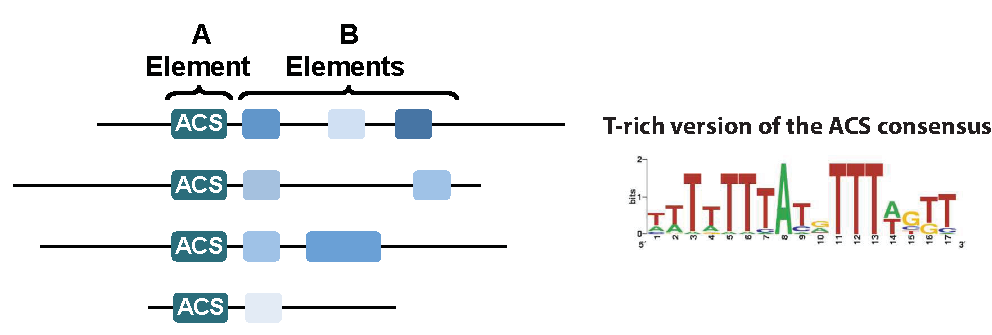
\includegraphics[width=\textwidth]{figures/results/acs}
\caption[ACS consensus and arrangement relative to other origin DNA elements]{Cartoon showing the most typical arrangement of sequence elements within origins. the ACS is required, while several B elements contribute to origin specification downstream of the T-rich strand of the ACS.}
\label{fig:originSchemaIntro}

\end{figure}

\paragraph{B elements}
A family of motifs with little sequence conservation, B elements are mainly AT-rich and always map downstream of the T-rich strand of the ACS (Fig. \ref{fig:originSchemaIntro}) \cite{raghuraman:2016:sequence}. 
While a match to the A element consensus is found in every origin \cite{celniker:1984:deletion}, no individual B element is universally required for origin activity \cite{marahrens:1992:yeast,lucas:2003:dynamics}. Collectively, however, B elements constitute a requirement for proper origin activity.

B elements were originally thought to facilitate DNA unwinding due to their AT-richness \cite{huang:1993:dna}. Subsequent studies, however, revealed that some B elements are playing a more active role, contributing to the recruitment of the replisome \cite{wilmes:2002:b2}.

\subsection{Nucleosome Positioning in Origins}
%\vspace{5mm}

Sequence elements are not enough to qualify an active origin. 
More than 10,000 matches for the ACS exist in the genome of S.cerevisiae, however, only 400 replication origins were identified. 
Moreover, it has been reported that some origins are able to efficiently drive replication of a plasmid, but are rarely used \invivo{} \cite{newlon:1993:analysis, santocanale:1999:activation}. 
Investigation of this context-dependent activity showed that nucleosome positioning plays a crucial role in origin activity and that functional origins \invivo{} are always associated with nucleosome free regions. 
In support of this notion, experiments forcing nucleosome assembly within the A or B elements resulted in abrogation of replisome assembly \cite{lipford:2001:nucleosomes}. 


The ACS itself was speculated to be able to drive nucleosome positioning, a notion supported by \invivo{} studies \cite{eaton:2010:conserved, berbenetz:2010:diversity}.
In these reports, the authors show that ACS sequences contained in active origins are surrounded by NFR, although formation of the latter is per se not sufficient to specify an origin as non-functional ACS are also associated with low nucleosome occupancy, albeit to a lesser extent.


Lastly, binding sites for transcription factors were detected within origins and, although their function remains somewhat unclear, are speculated to contribute to the maintenance of NFR within the origin \cite{diffley:1992:proteindna, rhode:1989:gene}. 
For example, the transcription factor Abf1 (ARS Binding Factor) is often found near origins and is known to recruit chromatin remodeling complexes to deplete nucleosomes at promoter regions. 
Studies on these origins showed that deleting Abf1 binding sites results in loss of activity, but replacing the sites with those of other transcription factors associated with NFR generation, such as Rap1, retains the replication activity \cite{marahrens:1992:yeast}.

\subsection{Transcription in Origins}

Multiple factors can affect the efficiency of an origin.  
For example, sequence elements can strongly contribute by affecting either ORC binding or pre-RC assembly. 
However, extrinsic factors such as nucleosome positioning can epistatically affect origin activity by occluding said elements \cite{bodmerglavas:2001:rna}. 
This raises the question: what other extrinsic processes can impact the initiation of replication? Several studies have investigated the effects of transcription on origin activity, but the results in the literature are controversial. 
While it generally agreed upon that transcription has a deleterious effect on origin activity \cite{tanaka:1994:transcription,nieduszynski:2005:requirement}, a substantial amount of evidence exist to argue that presence of RNAPII within origins can enhance their activity \cite{yankulov:1999:mcm,gauthier:2002:role}. 


Tanaka and colleagues originally investigated the problem by analyzing ARS1, an origin that partially overlaps with the gene TRP1. 
They observed that changing the endogenous promoter of TRP1 to a stronger one led to significant loss of origin activity \cite{tanaka:1994:transcription}.
A later study found that high transcriptional output across origins increases their sensitivity to ORC mutants (i.e. transcription increases loss of activity in the context of ORC mutations). 
The authors proposed a model according to which susceptibility to ORC mutants strictly depends on the intrinsic properties of each origin (e.g. sequence elements) but can be affected by extrinsic elements such as transcription \cite{nieduszynski:2005:requirement}. 


In seeming contradiction, several other studies demonstrated how RNAPII is capable of enhancing origin activity through its presence in the vicinity of the origin. 
In particular, the CTD of RNAPII was shown to interact with subunits of the replicative helicase MCM2-7 in both xenopus and human \cite{yankulov:1999:mcm}. 
Studies in yeast corroborated this result by showing that not only tethering of RNAPII CTD at replication origins can enhance activity, but also that cells with a shortened CTD (10 heptapeptide motifs in place of 26) show increased plasmid loss rates \cite{gauthier:2002:role}. 
Lastly, a recent study investigated origins associated with rDNA loci and concluded that RNAPII molecules participate to ORC binding to origins through their  ser2-Phosphorylated CTD \cite{mayan:2013:rnapii}. 


Although there are compelling arguments on both sides, mechanistic details are still lacking and current models cannot yet account for these discrepancies.

\section{Mechanisms of DNA replication}

Because of the importance of proper DNA replication for genome stability, its mechanism of action must ensure that the entirety of the genome is duplicated once and only once. 
In order to achieve this result, replication occurs in two discrete steps \cite{diffley:1994:two}.
The first step occurs exclusively in the G1-phase, and is called origin licensing.
During this step the six subunits Origin Recognition Complex (ORC) binds the ACS and associates with two ancillary factors named Cdc6 and Cdt1. 
When interacting, these three licensing factors are able to recruit multiple pairs of inactive replicative helicases around double stranded DNA, forming the pre-replication complex (Fig \ref{fig:repSteps}) \cite{gambus:2011:mcm27, remus:2009:concerted, seki:2000:stepwise, rowles:1999:changes, donovan:1997:cdc6pdependent}.
Replicative helicases are multisubunit complexes composed of MiniChromosome Maintenance proteins (MCM2 to MCM7). 
In S-phase, MCM2-7 will serve both as platforms for the assembly of other replisome components and as driving force for replicative fork elongation. 
It is important to note that during the first step of replication, only a subset of all origins are licensed. This subset is influenced by specific origin properties (e.g. strength of the ORC binding site, nucleosome occupancy etc.), but not deterministically chosen.

\begin{figure}[ht]

\centering
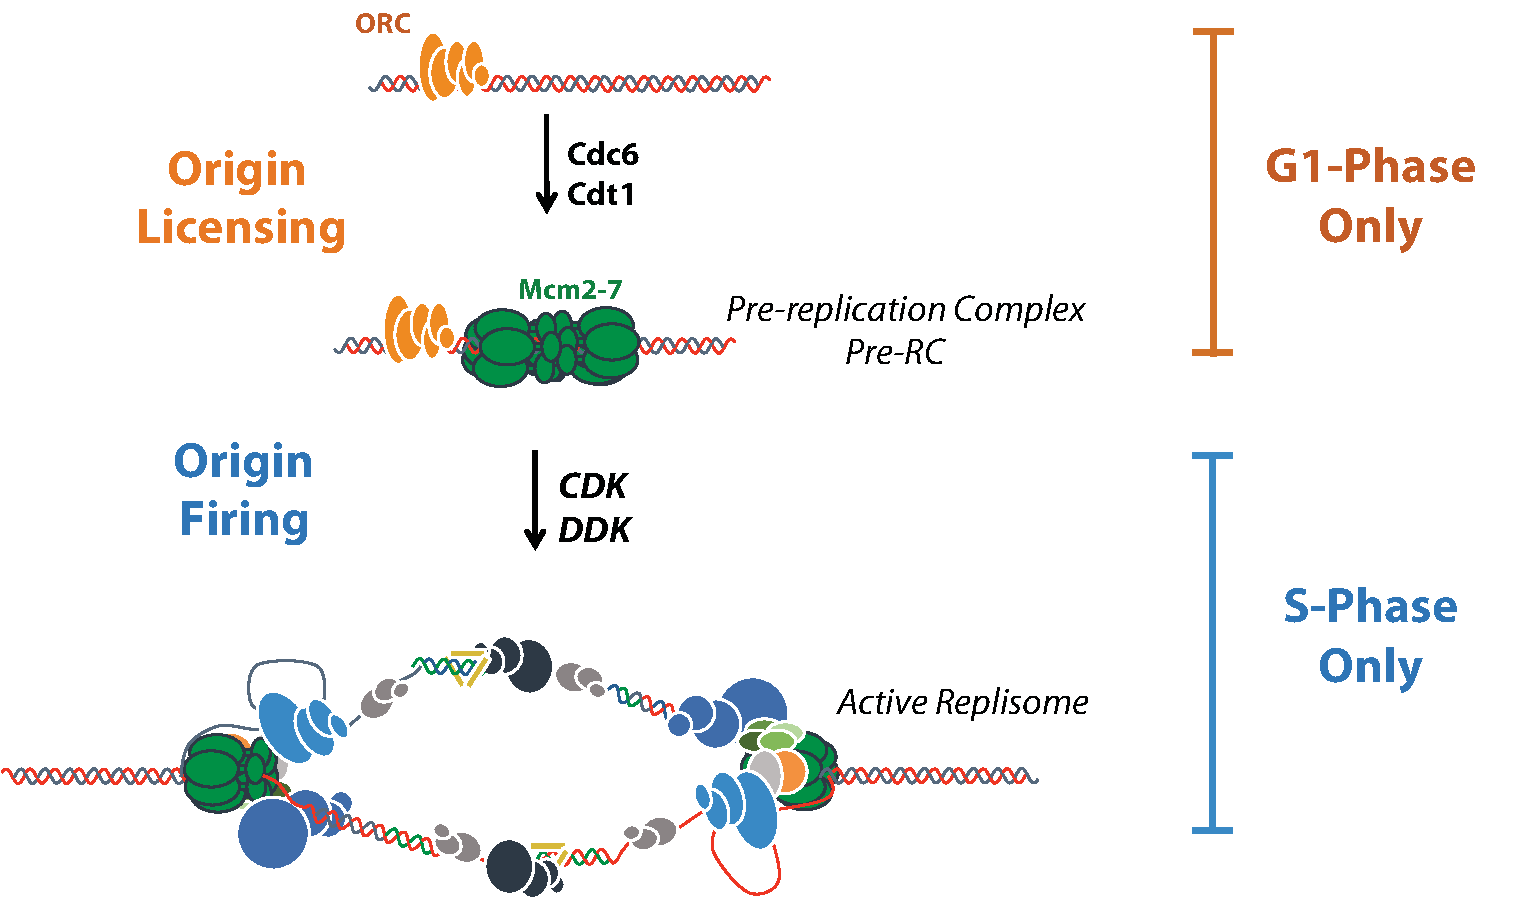
\includegraphics[width=\textwidth]{figures/introduction/repSteps}
\caption[Stepwise mechanism of DNA replication]{DNA replication takes place in two distinct steps. First ORC is required to bind to replication origins during the G1-phase and recruit the Pre-replication complex. Second, upon entry in S-phase, the pre-RC (among others) is phosphorylated and the full replisome can assemble and eventually fire.}
\label{fig:repSteps}

\end{figure}

The end of the G1-phase and the beginning of the S-phase marks the end of the licensing step and the beginning of the second step of DNA replication: the activation step. 
During this step, dormant pre-replication complexes at licensed origins activate, assemble into the active replisome and eventually fire. 
In order to prevent re-licensing of an already activated origin—and therefore avoid the risk of firing the same origin twice, leading to re-replication—the ORC complex is  inhibited through phosphorylation and MCM2-7 are rapidly depleted from the nucleus before this step begins \cite{nguyen:2001:cyclindependent}. 


Entry into S-phase coincides with a cascade of phosphorylation signals that activates the CDK and DDK kinase complexes. 
These cell cycle specific enzymes phosphorylate the pre-replication complex and are thought to induce structural rearrangements that allow assembly of the complete replisome. 
First the replicative helicases form the CMG complex (Cdc45-MCM-GINS) with Cdc45 and the GINS complex \cite{moyer:2006:isolation, aparicio:2009:human}. 
Subsequently, DNA polymerases pol $\delta$ and $\epsilon$ join the forming replisome. 
This allows the complete replisome to form and marks the start of fork elongation.
















\part{Results and Discussion}
	\boldchapter{Termination of RNA Polymerase II Through a Road-Block Mechanism}

In section \ref{roadblockIntro} I described how road-block termination is an effective tool in transcription termination of RNAPI at rDNA loci. 
At the beginning of my doctoral studies, the laboratory had found that road-block can also serve as a termination mechanism for RNA polymerase II, and that one of the molecular effectors of this phenomenon was the general regulatory factor Reb1. 
A major part of my thesis work was therefore dedicated to exploring the notion of road-block applied to RNA polymerase II through the use of genome-wide techniques.

This work led to the identification of other effectors of road-block termination and the better characterization of the genome-wide extent of this pathway. 
The work is summarized in two manuscripts presented below. 
The first describes road-block termination elicited by Reb1 and mechanistically characterizes the pathway.
The second identifies other effectors of road-block and further explores its genome-wide extent.

\singlespacing
\section{Road-Block Termination by Reb1 Restricts Cryptic and Readthrough Transcription}
\doublespacing

In this work, I focused on the genome-wide characterization of road-block termination. 
Previous work form the group had identified specific hallmarks of road-block in synthetic sequences, such as the accumulation of RNAPII about 15-20 nucleotides upstream of Reb1 binding sites. 
I therefore used genome-wide RNAPII occupancy datasets to probe Reb1 binding sites on the genome and determine whether they are associated with polymerase pausing. 
In order to achieve this, I devised an algorithm able to identify peaks of polymerase pausing and their position relative to Reb1 binding sites. 
Additionally, I analyzed a set of synthetic sequences known to elicit Reb1-dependent road-bock termination in order to expand the binding consensus for Reb1. 

\clearpage


\includepdf[pages={1-},scale=0.75]{papers/reb1+sup.pdf}

\clearpage

\singlespacing
\section{Genomewide Analysis of Road-Block Termination}
\doublespacing

Following the publication of Colin \textit{et al.}, I focused on the possibility that other DNA binding proteins might be effectors of road-block termination \invivo{}. 
Besides Reb1, Rap1 had also been identified as a possible road-blocking factor from previous experiments. 
This led me to investigate the family of General Regulatory Factors, which resulted in the identification of several other possible road-blocking factors belonging to this class, such as Abf1. 
Using a combination of already published datasets and newly generated data, I applied meta-gene analyses and other computational techniques to identify genomic loci associated with polymerase pausing and termination events. 


\clearpage


\subsection{Introduction}

The compact genome of S.cerevisiae is covered by several machineries that need to be temporally and spatially coordinated to limit interferences that might affect robust reading and perpetuation of the genetic information. Transcription itself best exemplifies the complexity of the genomic landscape. Transcription initiation occurs frequently in regions and direction that largely overrun the annotations of genes with an assigned function. This is believed to be due to a leaky control on initiation and to the general of bi-directionality of promoters, which is also generally conserved in evolution. Transcription units largely overlap in both sense and antisense direction, and although RNA polymerases II (RNAPII) only seldom collide [Zenklusen], the chromatin marks associated with ongoing transcription persist, and are susceptible to considerably impact concurrent transcription events. Overlapping transcription has also a large potential for regulation of gene expression, which is controlled and sometimes tamed to the need of the cell. 

The pervasive nature of transcription brings about two main potentially perturbing elements: the first is the presence of transcribing RNA polymerases which might directly affect other DNA-related events; the second is the production of many non-coding RNA molecules that might titer RNA-binding factors and indirectly affect gene expression. Cells possess tools to control both, by terminating “spurious” transcription events and degrade a large fraction of the RNA produced. In this perspective, transcription termination and RNA degradation, besides being devoted to the production of functional RNAs, additionally qualify as quality control mechanisms. 

In yeast, two main pathways of termination exist. The first is operated by a complex called the Cleavage and Polyadenylation Factor-Cleavage Factor (CPF-CF) and is used to arrest transcription of mRNA coding genes. The CPF-CF complex recognizes signals on the nascent RNA and cleaves it, producing a 5’ fragment that is polyadenylated by the Pap1 poly(A) polymerase and exported to the cytoplasms.  The 3’-fragment still associated to the transcribing polymerase is recognized and degraded by a 5’-3’ exonuclease,  Rat1, which contributes to dismantling the elongation complex by a much discussed but still unclear mechanism. The CPF-CF is also believed to be directly involved in termination by allosterically modifying the properties of the transcription elongation complex. 
The second canonical pathway is dependent on the NNS (Nrd1-Nab3-Sen1) complex and was traditionally associated to the production of sn- and snoRNAs. Nrd1 and Nab3 bind the RNA at short motifs containing a well-conserved 4-5 nucleotides core and are thought to recruit Sen1 that translocates on the nascent RNA to release the polymerase by a mechanism that remains unclear. Peculiar to this pathway is the treatment of the RNA released, that is polyadenylated by a different poly(A) polymerase, Trf4, functioning within the TRAMP4 (Trf4-Air2-Mtrf4-Polyadenylation) complex, and trimmed to its mature size in the nucleus by the exosome, a large multisubunit complex that is endowed with 3’ to 5’ exonuclease activities. 

A large share of the transcripts produced by pervasive transcription do not code for proteins and to what extent these RNAs have specific functions remains matter of debate. They are sorted in classes, generally defined by the pathways associated to their metabolism. CUTs (Cryptic Unstable transcripts) have been first described based on their extreme instability. These RNAs derive from transcription events terminated by the NNS pathway and are degraded to completion by the TRAMP-exosome pathway. When NNS termination is defective, elongated forms of CUTs are produced that are presumably terminated downstream by the CPF-CF pathway because they are insensitive to nuclear, exosomal degradation. These elongated forms of CUTs have been more recently named NUTs (Nrd1 Unterminated Transcripts).  Some of the non-coding RNAs produced by pervasive transcription are sufficiently stable to be detected in wild type cells (SUTs, stable unannotated transcripts) or are degraded in the cytoplasm by the nonsense-mediated decay (NMD) and Xrn1 pathways (XUTs, Xrn1-sensitive Unstable Transcripts). Finally, some are only detected in particular physiological conditions (MUTs,  meiotic unannotated transcripts). 

We have recently described an additional pathway of transcription termination that depends on the DNA-binding protein Reb1 and that was dubbed roadblock (RB) terminaition. The elongating polymerase was shown to pause upstream of DNA-bound Reb1, which provokes its release by a mechanism that involves its ubiquitylation and presumably degradation. The isolated binding site of Reb1 was shown to be sufficient for eliciting termination when inserted in regions of active elongation, indicating that additional sequence elements are not required for efficient RB termination.  Because, akin to CUTs, the RNAs released are polyadenylated by TRAMP and degraded by the nuclear exosome, these transcripts where dubbed RUTs (Reb1-dependent Unstable Transcripts).  

In this report we demonstrate that several DNA-binding factors or complexes are able to terminate transcription by a RB mechanism. We generated high-resolution data on the distribution of RNAPII upon depletion of RB factors to address the significance and extension of RB termination at the genomewide scale.  We demonstrate that prominent peaks of roadblocked polymerases accumulate in intergenic regions immediately downstream of canonical terminators, indicating the significant occurrence of transcriptional readthrough in wild type cells. Akin to the leaky control on transcription initiation, the constitutive failure to terminate efficiently generates an additional level of pervasive transcription that has the potential to strongly affect the function of downstream regulatory regions or other DNA associated events. 
We show that RB and canonical termination pathways are not dependent on each other. High resolution analyses of RNAPII occupancy upon affecting either RB or CPF-CF and NNS termination indicates that RB is unlikely to partake in canonical termination and, conversely, that NNS and CPF-CF pathways are unlikely to be involved in RB termination. Rather, RB termination plays an important quality control role in limiting pervasive transcription events due to termination failure.  
The faculty of DNA associated factors to alter the processivity of elongation complexes, and the widespread occurrence of these factors defines a large potential in shaping and regulating the transcriptome. We propose that roadblock termination constitutes an additional, general level of control on transcription that operates at the post-initiation level by altering the efficiency and extent of RNAPII elongation. 

\subsection{Results}

\singlespacing
\subsection*{\textit{In Vivo} Selection Reveals Rap1-Dependent Transcription Termination}
\doublespacing

We have previously described a procedure to select transcription terminators from pools of naïve sequences [REF]. Briefly, test sequences are inserted within a transcription unit driven by the tetracycline-repressible (TetP) promoter, roughly 200nt downstream of the transcription start site. A second promoter from the GAL1 gene is inserted downstream and drives expression of a selectable marker, CUP1, the expression of which is required for yeast growth in copper-containing medium. In the absence of a terminator in the test sequences, transcription driven from TetP silences the GAL1 promoter by transcription interference and prevents CUP1 expression, which leads to copper-sensitivity. When the test sequence induces termination, the CUP1 gene is expressed and yeasts grow on copper-containing plates. 

Using this system we selected terminators from a pool of sequences containing a stretch of 120 random nucleotides. We selected many sequences inducing termination via the NNS pathway and via the Reb1-dependent roadblock pathway. We also selected sequences that do not belong to either class, some of which contain a motif resembling a Rap1 binding site (Figure 1b). Rap1 recognizes its site via a Myb-like DNA-binding domain and is involved in many DNA-associated processes, including telomere maintenance and gene expression. Rap1 is also strongly associated to the positioning and formation of nucleosome free regions (NFR). 

It has previously been shown that the presence of a Rap1 binding site can induce RNAPII stalling in a model Ty1 retrotransposon construct (Yarrington et al, 2012). In this study, the occurrence of Rap1-dependent transcription termination was ruled out based on the analysis of the transcripts produced in the presence of the Rap1 site. These RNAs were non-adenylated and insensitive to nuclear degradation, and therefore assumed to be nascent RNAs associated to the stalled polymerase. Moreover, it was not demonstrated that stalling is dependent on the integrity of Rap1 or its binding to the DNA.
The stalling model would hardly be compatible with our results, because only loss of polymerases – and therefore termination – is expected to prevent transcription interference. We therefore assessed whether the presence of the selected site would induce Rap1-dependent transcription termination. We first demonstrated that the Rap1 binding site is necessary and sufficient to prevent transcription interference at the GAL1 promoter. Indeed, mutation of the site in the context of a selected clone prevented yeast growth on copper, while insertion of the site in a fragment of the coding region of the HSP104 gene was sufficient to induce copper resistance (supplementary figure 1).  

These results were confirmed by direct analysis of the RNA produced. To assess whether the transcripts released undergo nuclear degradation, we analyzed the RNAs in both a wt and degradation-defective rrp6∆ and trf4∆ strains. As shown in figure 1C, an RNA of the expected size is produced when a selected terminator is present in the reporter construct. For all of the terminators analyzed, the size of this RNA is XXnt shorter than the distance between the transcription start site and the Rap1 site (data not shown), suggesting that stalling or release of the polymerase occurs upstream of the site, which is consistent with a roadblock mechanism. 

The transcripts produced are strongly sensitive to degradation, as indicated by their marked steady state increase when the analysis is performed in a ∆rrp6 exosome mutant (Figure 1C, lanes 1-2). This indicates that these transcripts cannot solely correspond to polymerase-associated nascent RNAs but rather that they are released upon transcription termination. The short transcript disappears to the profit of a longer, read-through product when the Rap1 site is deleted (compare lanes 3 and 4) The bulk of the transcripts released and degraded appears to be non-adenylated (Figure 1C, compare lanes 7, 10 and 13), although a fraction is polyadenylated by Trf4 (compare lanes 9 and 12). The transcripts that are detected in a wild type strain are non-adenylated (lanes 5-7) and might correspond to nascent RNAs that are protected from degradation because of their association with the polymerase.

The dependency on the Rap1 site strongly suggests, but does not prove that Rap1 is involved in termination. Indeed, termination might occur via other pathways, e.g. as a result of the recognition of partially or fully overlapping signals at the Rap1 site.  To prove the Rap1 dependency, we transiently depleted this essential factor with the anchor away strategy and analyzed the transcripts produced. As shown in figure 2A, the levels of the short RNA derived from the reporter construct are markedly decreased in the absence of Rap1, to the profit of a longer species earmarking termination at a downstream site [REF]. From this result we conclude that Rap1 is necessary to induce termination at the selected sites. 

Finally, we have previously shown that release of the roadblocked polymerase from the DNA template occurs following its ubiquitylation that depends on the Rsp5 ubiquitin ligase. When the elongation complex is dismantled, the RNA released is polyadenylated and degraded rapidly; conversely, the persistence of roadblocked RNAPII on the DNA template following mutation of Rsp5 leads to an increase of the nascent, non-adenylated transcript that can be detected in a wild type strain [REF]. Northern blot analysis confirmed the expected increase in the levels of nascent RNAs when the Rap1-roadblocked polymerase is less efficiently removed in a thermosensitive rsp5-1 mutant strain (figure 2B). 

This finding is also substantiated by the observation that recombinant Rap1 binds very efficiently the double stranded DNA but not the RNA or single stranded DNA version of its site (figure S2). 

Together, these results demonstrate that transcription termination occurs by a roadblock mechanism at sites bound by Rap1. 

\singlespacing
\subsection*{Rap1-Dependent Transcription Termination in the \cer{} genome}
\doublespacing

These results constitute the proof-of-principle that transcription termination can occur in a Rap1-dependent manner, but do not prove that it occurs significantly in the S. cerevisiae genome. A hallmark of roadblock termination is the accumulation of RNAPII immediately upstream of the site of roadblock, due to polymerase pausing. 

We therefore assessed whether RNAPII pausing can be observed in the S.cerevisiae genome   at Rap1 sites and whether pausing would be dependent on Rap1. To this end, we analyzed the RNAPII distribution in a wild type and a Rap1 anchor away (Rap1-AA) strain by a modified crosslinking and cDNA analysis (CRAC) method [REF]. By this approach, the position of the polymerase is directly inferred by sequencing the nascent transcript associated to the largest subunit of the enzyme after in vivo UV crosslinking (RNAPII-CRAC, Tollervey Milligan). Consistent with the notion that the signals obtained genuinely represent nascent and not mature transcripts, intronic regions where largely covered in the RNAPII CRAC dataset but not in the sequencing of mature, total RNAs (Figure S3).

In the Rap1-AA strain, Rap1 is rapidly and efficiently depleted from the nucleus upon addition of rapamycin [REF].  Notable examples of sites of Rap1-dependent roadblock sites are shown in figure 3. Two Rap1 binding site are present upstream of the HYP2 gene and constitute a prominent site of Rap1 localization as detected by several techniques [cite ChIP exo and D. Shore]. CRAC analysis reveals a prominent accumulation of the RNAPII signal immediately upstream of the Rap1 sites, indicating pausing. The occurrence of termination is demonstrated by the existence of a non-annotated unstable transcript ending in correspondence of the RNAPII peak, revealed by microarray analysis [Neil et al.] and by a cluster of 3’-end SAGE [Figure 3A, Neil et al.]. RNAPII pausing and termination were Rap1-dependent, because depletion of Rap1 led to a strong reduction in the RNAPII peak and to the appearance of a readthrough signal downstream of the site (figure 3A, inset). Finally, insertion of the two Rap1 sites in the heterologous context of our reporter system induced Rap1-dependent termination and led to the production of an unstable RNA (figure S4).

Two other examples are shown in figure 3B-C. In these cases, the Rap1 occupancy site is located between two tandem genes and the accumulation of RNAPII is most likely due to transcription events reading through the upstream terminator (see below). In both cases, depletion of Rap1 leads to abrogation of the peak and increased RNAPII signals downstream of the site (Figure 3B-C, insets). 

To extend these results to a genomewide perspective we profiled the average distribution of the RNAPII CRAC signal around aligned sites of Rap1 occupancy found in promoter regions.

Rap1 is required for the strong expression of ribosomal protein (RP) genes, and is often positioned in nucleosome free regions (NFRs) upstream of these genes. Consistently, a major peak of RNAPII occupancy is observed downstream of the aligned Rap1 binding sites, corresponding to the occurrence of transcription initiation within a relatively short window (figure 4A). Importantly, however, a significant peak demonstrating RNAPII pausing is also observed upstream of Rap1 binding, which is associated to the occurrence of transcription termination in the same region (see below). Importantly, sequestering Rap1 out of the nucleus led to a significant decrease in the RNAPII pausing peak demonstrating that Rap1 dependent roadblock occurs at many sites of Rap1 binding in the genome.

Similar RNAPII CRAC analyses were also performed upon Reb1 depletion. Peaks of RNAPII pausing were readily observed at individual sites of Reb1 occupancy that disappeared upon Reb1 depletion (figure S5 and data not show). Because Reb1 is also required for the expression of many genes, profiling RNAPII distribution around aligned sites of Reb1 occupancy revealed a similar transcription initiation peak as for Rap1 (figure 4).  Importantly, a prominent peak indicating RNAPII pausing was also observed upstream of Reb1 that strongly decreased upon sequestering Reb1 out of the nucleus. Overall, these results demonstrate the significant occurrence of Rap1- and Reb1-dependent, roadblock transcription termination in S. cerevisiae.


\singlespacing
\subsection*{Widespread Redundancy in Transcription Termination}
\doublespacing

In the compact S. cerevisiae genome, efficient and timely release of the elongation complex is essential to prevent interference between contiguous transcription units. Whether CPF termination is inherently highly efficient or enforced by redundant mechanism remains unclear. Many sites of Reb1 and Rap1 occupancy are located in intergenic regions, downstream of genes terminated by the CPF pathway. If significant transcriptional read through occurs at these CPF terminators, polymerases are expected to be roadblocked at downstream sites of Reb1 and Rap1 occupancy, as also suggested in the cases of PIL1 and ALD5 (figure 3B-C). We therefore restricted our metasite analyses to Reb1 and Rap1 occupancy sites located within 300nt downstream of mRNA-coding genes. In these conditions, only polymerases escaping termination (if any) are expected to contribute to the metaprofile observed. As shown in figure 4B, transcriptional roadblock is clearly observed in the wild type strain at sites of Rap1 and Reb1 occupancy downstream of canonical CPF terminators. To prove that roadblocked polymerases indeed originate from readthrough at upstream terminators and not from spurious initiation between terminators and the roadblock sites, we also performed a parallel RNAPII CRAC analysis using a thermosensitive rna15-1 allele, which impairs CPF termination.  A prominent increase in the roadblock peak was clearly observed upon impairing CPF termination in the rna15-1 mutant, consistent with the notion that the flux that aliments roadblocked polymerases originates from upstream transcription units and increases when upstream termination is defective. As a control, we profiled RNAPII distribution at the same set of genes using published PAR-CLIP data obtained [] upon nuclear depletion of Nrd1, an essential actor of NNS termination that is not involved in termination of mRNA coding genes. In these conditions we did not observe an increase in the roadblock peak (figure S6 and data not shown) confirming that roadblocked polymerases originate from upstream, CPF-dependent genes. 
Although less prominent, roadblock was also observed at sites of Abf1 occupancy downstream of CPF terminators, which increased, as for Rap1 and Reb1, when termination was impaired in an rna15-1 mutant (figure S7). 

Overall, these results demonstrate the widespread occurrence of significant levels of transcription readthrough at CPF terminators in strains that are proficient for transcription termination. This results in the constitutive accumulation of roadblocked polymerases at sites of Rap1 and Reb1 occupancy (and many additional sites in the genome, see below).


\singlespacing
\subsection*{Roadblock is not Part of the CPF Termination Mechanisms}
\doublespacing


Although these results strongly suggest that roadblock termination acts to neutralize transcriptional readthrough downstream of CPF-dependent terminators, it cannot be excluded that roadblocking the polymerase is an important requirement for efficient termination at the upstream canonical sites. For instance, it can be envisioned that pausing induced by the roadblock favors chasing of the polymerase by Rat1. In this perspective, it is expected that reducing the roadblock should affect the efficiency of termination at the upstream sites. To address this possibility, we investigated whether increased transcriptional readthrough could be observed at CPF terminators in the absence (or strong reduction) of the downstream roadblock. We analyzed the level of polymerase in the region immediately downstream of CPF terminators in Reb1 or Rap1 anchor away strains upon nuclear depletion of either factor. Three examples of CPF-dependent genes with a downstream roadblock are shown in figures S8. In all occurrences, transcription termination occurred efficiently at the CPF sites even in the absence of the roadblock as witnessed by a very similar RNAPII signal at and downstream of the termination region. 

To generalize these observations, we first compared the RNAPII metaprofiles in regions of CPF termination upstream of a Rap1 binding sites in the presence and absence of the roadblock factor. To this end we aligned for each gene the strongest site of poly(A) addition as defined by TIF-seq analyses [Steinmetz], trusting that this will allow a sufficiently precise approximation of the average termination region. A decrease in the average RNAPII signal was observed in wild type cells in this region, confirming the progressive occurrence of termination. Depletion of Rap1 had no impact on the distribution of the RNAPII signal that declined in the termination region very similarly to the wild type indicating identical efficiencies of termination at the upstream CPF sites (Fig. 5). As a control, a termination defect could clearly be observed in rna15-1 cells at the non-permissive temperature. Similar results were obtained for the set of CPF-dependent genes upstream of a Reb1-dipendent roadblock (data not shown). 

To substantiate these results we calculated the fractional level of readthrough for each CPF-dependent gene upstream of a Rap1- dependent roadblock by dividing the density of reads in the termination region by the density in the gene body. The distribution of the values obtained is strongly affected by the rna15-1 mutation, as expected for a bona fide termination defect (p=1E-8), but not by the absence of Rap1, demonstrating that the roadblock does not significantly impact CPF termination. 

\singlespacing
\subsection*{Roadblock and NNS-Dependent Termination}
\doublespacing

While this work was in progress another study suggested that roadblock- and NNS-dependent termination are functionally linked, notably that: i) roadblock is part of the mechanism of snoRNA termination and ii) that roadblocked polymerases are released by the NNS pathway. This study relied on the analysis of transcripts produced in different mutant conditions and on the published distribution of polymerases in wt and Nrd1 anchor away strains []. We undertook to revisit this important question using our high-resolution RNAPII CRAC in cells defective for the CPF, NNS and roadblock pathways. 

Roadblock peaks have been shown to increase in strains defective for NNS termination, which was interpreted as evidence of defective clearing of roadblocked polymerases when NNS termination is impaired []. An alternative interpretation, which we favor, is that when NNS termination is defective, polymerases that do not terminate at primary NNS termination sites accumulate downstream at roadblock sites.  Consistent with this notion is the finding that the level of roadblocked polymerase is not sensitive to NNS termination at roadblock sites preceded by CPF terminators (figure S6). Two such examples are shown in figure 6. The RNAPII roadblock peak increases considerably when CPF termination is impaired at the PIL1 and ALD5 loci but is unaffected by depletion of NRD1. Identical results were obtained at these loci when Sen1 was depleted (data not shown). Conversely, depletion of Nrd1 leads to an increase of the roadblock peaks at Reb1 and Rap1 sites located downstream of NNS terminators (figure S9). Together, these results indicate that roadblocked polymerases are not generally released by the NNS pathway. 

In a small number of snoRNAs the roadblock is located very near to the NNS terminator and it is possible that it contributes to the formation of a functional RNA. We analyzed the polymerase profile around four of these snoRNAs for which a Reb1- (SNR161, SNR8, SNR48) or Rap1-dependent (SNR39B) roadblock peak of variable intensity was observed in the termination region. Depletion of Nrd1 led to a clear increase of the roadblock peak, as expected. However, a clear increase in RNAPII occupancy was also observed between the NNS terminator and the region of the roadblock (figure 7, red arrowheads), indicating the existence of a readthrough at the primary terminator that feeds the flow of polymerases accumulating later at the roadblock. This was clearly visible at the SNR8 and SNR48 loci, where the roadblock is slightly more distal (figure 7, panels A-B), but also observed at SNR161 and SNR39B where the signal due to the readthrough increase somewhat merged with the roadblock peak (figure 7 C-D).

Conversely, no evidence of readthrough could be observed at the primary termination site when the roadblock factor (Rap1 or Reb1) was depleted, which only led to the expected decrease in the roadblock peak.  A small but clearly visible readthrough extended downstream of the roadblock (figure 7 blue arrowheads), most likely due to the release of polymerases accumulating at the failsafe site.   

We also analyzed the RNAs produced in the absence of the roadblock (figure 7). We depleted Reb1 or Rap1 in an rrp6∆ strain, which allowed visualizing the primary product of transcription that is stabilized in this genetic context. Interestingly, in spite of the overall low level of polymerases going through the roadblock site in the absence of Reb1 or Rap1, a significant increase in the amount of pre-snoRNA was generally observed (figure 7, see the RNAseq profiles at SNR8, SNR161 and SNR39B loci; data not shown), suggesting that transcription events terminating downstream of the roadblock produce transcripts that are generally more stable than those produced by transcription terminating at the primary (NNS) or secondary (roadblock) terminator. The levels of the mature snoRNAs were generally increased or unchanged in the absence of the roadblock (data not shown), although the general stability of these forms prevents from drawing strong conclusions in these transient depletion experiments.  

These experiments strongly suggest that the absence of the roadblock does not prevent the production of functional snoRNAs but allows the production of stable transcripts derived from a low level of readthrough transcription at the primary NNS terminator. Importantly they strongly support the notion that roadblock termination functions as a fail-safe mechanism for both the CPF and the NNS pathways.


\singlespacing
\subsection*{Functional Importance of Fail-Safe Transcription Termination }
\doublespacing

As shown in figure 8, depletion of Rap1 strongly downregulates transcription of RPL11B and RPS24A. These genes are positioned downstream of a Rap1-dependent roadblock where polymerases derived from upstream transcription accumulate. Removal of the roadblock allows the progression of these polymerases into the downstream promoters (figure 8), which they might silence by transcriptional interference. However, it is also possible that Rap1 directly promotes transcription activation of these genes, independently of its role in roadblocking upstream polymerases. To distinguish between these (non exclusive) possibilities we investigated whether maintaining the sole “protective” function of Rap1 would be sufficient to restore expression of the downstream genes. To this end we depleted Rap1 in cells expressing the well-characterized DNA binding domain of Rap1 (Rap1-DBD, aa. 358-601), which is not expected to activate transcription. As a control, we also expressed the wild type Rap1 or an empty plasmid upon endogenous Rap1 depletion, and analyzed the RNA produces by RNAseq. Prior RT-qPCR analyses demonstrated that expression of Rap1-DBD is sufficient to restore the roadblock upstream of HYP2 (Fig. S10 and data not shown). The overall impact on the transcriptome of Rap1-DBD will be extensively discussed elsewhere (Challal et al., in preparation), but the RPL11B and RPS24A RNA profiles, together with RNAs derived from neighboring genes as a control, are shown in figure 8. Consistent with the RNAPII CRAC data, expression of RPL11B and RPS24A is markedly affected by the depletion of endogenous Rap1 and restored by the concomitant expression of wt Rap1. Importantly, expression of the DNA binding domain alone of Rap1 is sufficient to restore RPL11B and RPS24A to wild type levels. This is not due to a generalized ability of Rap1-DBD to activate Rap1 target genes as demonstrated by the failure of Rap1-DBD to restore expression of RPS0A (figure 8C) or RPL29 (data not shown).

Together these results support the notion that the constitutive readthrough at CPF (and possibly NNS) terminators can be sufficient for silencing downstream genes, underscoring the importance of the protective action of roadblock factors.  

\singlespacing
\subsection*{Extensive roadblock Termination in the \cer{} genome}
\doublespacing

In the light of the results shown here on Rap1 and Reb1, we undertook to assess more generally the occurrence of roadblock termination at sites of occupancy for DNA-binding proteins or complexes. For a more stringent and sensitive meta-analysis, we plotted the median level of polymerase occupancy at each position before a given site, which better reflects changes in the whole distribution of occupancy values. Indeed, the appearance of a peak at a given position is more stringently linked to changes that affect the whole distribution of values and less dependent on the contribution of extreme values. Consistently, a prominent and specific peak of polymerase pausing was observed by this method immediately upstream of many transcription factors (figures 9).  Roadblock occurs at a variable distance between 20 and 40 nucleotides upstream of the protein binding site, likely reflecting the topology of the collision between polymerase and the DNA-bound factor or complex of factors. 

We also sought evidence of roadblock termination at other sites where RNAPII transcription might collide with DNA-associated events. Prominent levels of roadblock termination were observed at centromeres and tRNAs. In S. cerevisiae, centromeres are defined by a set of short, conserved sequence elements located in a 125nt region. These sequences, CDEI, CDEII and CDEIII (figure 10) are specifically bound by DNA binding complexes that overall constitute the kinetochore, required for the attachment of the chromosomes to microtubules during cell division [REF, review]. The analysis of the RNAPII metaprofile around centromeres clearly indicates a prominent level of roadblock when centromeres are aligned using the external CDEI or the CDEIII sequence motifs, bound respectively by Cbf1 and the Cbf3 complex. 

Prominent levels of roadblock termination also occur at tRNAs. This was previously observed in the 5’-end of a model tRNA, where roadblock was attributed to the binding of the RNAPIII factor TFIIIB [REF]. We extended this finding genomewide, by showing RNAPIIs piling up at position -75 from the tRNA start site, corresponding to a roadblock induced by TFIIIB bound at position -50 from the start site. Importantly, however, we also observed a prominent roadblock antisense to the tRNA. RNAPII strongly accumulates about 50 nucleotides upstream of the annotated end of the tRNA (figure 11). Because RNAPIII transcription is not known to depend on factors bound to the DNA, we infer that roadblocking occurs from the collision of RNAPII with RNAPIII, presumably paused at the termination signal or persistently occupying the tRNA transcription region. 

Together, these data demonstrate that roadblock termination is not restricted to Reb1 or Rap1 binding sites, but also occurs at many different locations in the yeast genome. Aside from operating a quality control mechanism on the efficiency of termination at canonical sites, roadblock pausing of polymerases has potential for gene regulation and coordination of transcription with other DNA related events

\subsection{Discussion}


In a previous study we have described an additional pathway whereby transcription termination occurs when the elongation complex encounters the factor Reb1 bound to the DNA. Based on a few model cases we have proposed that roadblock termination by Reb1 limits pervasive transcription and functions to “protect” promoters regions from “invading” polymerases. The general validity of these concepts was, however, not addressed in this early study. Here we extend these concepts to a genomewide perspective and to other factors, providing a general view of the impact and functional significance of roadblock termination in the S.cerevisiae genome.  

We first demonstrated that Rap1, a DNA binding factors that has roles in transcription activation, gene silencing and telomere homeostasy, is also a roadblock factor. An earlier study showed that the fortuitous introduction of a Rap1 site in a Ty1 retrotransposon led to RNAPII stalling and repression of gene expression Based on the analysis of the RNA produced, which was non-adenylated and insensitive to exosome degradation, it was concluded that termination of transcription did not occur in these conditions [Yarrington]. We show that roadblock termination occurs upstream of Rap1, leading to the production of RNAs that are polyadenylated by Trf4 and degraded for a large part by the nuclear exosome. We also detected non-adenylated RNAs, which most likely represents the nascent RNA associated to the polymerase that pauses before termination. Importantly, nuclear depletion of Rap1 prevents termination, indicating that the protein – and not the presence of termination signals overlapping its binding site – is responsible for ending transcription. Failure to detect the polyadenylated fraction for technical reasons in the study by Yarrington et al. might account for the discrepancies; alternatively, termination might not occur in the Ty1 retrotransposon model for unknown reasons.


\singlespacing
\subsection*{The Mechanism of Roadblock Termination}
\doublespacing

Similar to what previously shown for Reb1 [Colin], release of the polymerase stalled upstream of the roadblock occurs, at least partially, as a consequence of its ubiquitylation by Rsp5 and presumably degradation. Thus, this pathway is not restricted to Reb1-dependent termination and presumably extends to all cases of roadblock, in addition to events of pausing that cannot be resolved in a more “conservative” manner as previously demonstrated for polymerases encountering a DNA damage [Svejstrup]. Using high resolution RNAPII occupancy data we observed very sharp peaks of stalling at the roadblock sites, which is hardly compatible with more than one polymerase roadblocked, on average, at a time. This indicates that the clearance due to the Rsp5 pathway is as efficient as the building up of the peak, at least at steady state.

It has been recently proposed that the NNS pathway is required for releasing roadblocked polymerases. This claim was essentially funded on the observation that i) Nrd1 and Nab3 binding sites are frequently present at sites of roadblock and ii) that peaks of polymerase stalling increase upon depletion of Nrd1 from the nucleus, which was taken as evidence that the clearance of roadblocked polymerases is affected when NNS termination is defective. Data shown in this report and in our previous study on roadblock termination are not compatible with this model. The strongest counterevidence is that the insertion of an isolated Reb1 [Colin et al.] or Rap1 site (this report) in a segment of the HSP104 gene lacking NNS termination signals, is sufficient for efficient RB termination. Moreover, these or similar constructs have been shown to be largely insensitive to depletion of Nrd1 and Nab3 [Colin et al.; data not shown]. 

This notion also holds for the natural cases of roadblock termination in the S. cerevisiae genome. We show that the cumulative RB peak significantly increases upon depletion of Nrd1 only when considering roadblock sites downstream of NNS, but not CPF-CF terminators (figures XX and YY). Conversely, when the RB sites are downstream of CPF-CF terminators, mutation in the CPF-CF complex (but not Nrd1 depletion) increase the levels of roadbocked polymerases (figures XX and YY).  This suggests that alterations in the NNS (or CPF-CF) complexes do not affect the clearance of roadblocked polymerases, but their further accumulation upon failure to terminate at upstream NNS- (or CPF-CF) dependent genes. 

Thus, we favor a model according to which roadblock termination operates independently of the NNS and CPF-CF pathways and does not allow recycling of the polymerase for further steps of transcription but leads to its degradation, together with the RNA that is produced. Such a disruptive mechanism might look uneconomical, but the concept is analogous to the seemingly useless transcription of many non-functional RNAs that are degraded rapidly after production by processing or quality control mechanisms. The energetic balance might still be favorable if the evolutionary cost of developing highly efficient, error-proof machineries is taken into consideration. In this respect, the genomewide analyses reported here strongly suggest that roadblock termination is unlikely to be devoted to the generation of functional molecules, but rather to controlling a relatively low fraction of polymerases that might significantly affect the efficiency or robustness of neighboring processes.


\singlespacing
\subsection*{Functional Significance of Roadblock Termination}
\doublespacing

We have previously proposed that in a few model cases, Reb1-dependent roadblock termination functions to neutralize transcription events that failed to undergo termination at upstream genes. The question addressed here is to what extent this is general, i.e. does significant transcription readthrough occur at CPF and NNS terminators genomewide and in cells that are proficient for termination. We show here that prominent roadblocks at Reb1 and Rap1 sites can be fed by polymerases that escape upstream CPF-CF and NNS-dependent termination, demonstrating the occurrence of constitutive readthrough at canonical terminators. Because we show that many DNA binding factors can roadblock, to different extents, the elongation complex, polymerases overlooking canonical termination signals run into “bumpy” roads that limit their progression in intergenic regions, where they could interfere with transcription initiation or other cellular processes. The genomewide analysis of RNAPII distribution in mutants of the CPF pathway show that in most instances, readthrough polymerases accumulate in the adjacent intergenic regions, which is fully consistent with this notion (unpublished results, or Challal et al., in preparation). 

A large wealth of evidence exists demonstrating that pervasive transcription is generated to a large extent by the leaky control of chromatin on initiation. This is particularly important for restricting the inherent bi-directionality of promoters and directing preferential initiation towards functional genes [Churchmann]. Mutation of many chromatin remodelers or modifiers further weakens such a repressive control on initiation [Churchman, Buratowski, others]. Leakiness in transcription termination is functionally analogous to the limited control of chromatin on initiation, in terms of the generation of pervasive transcription. In both cases, this allows transcription elongation in regions that are not necessarily producing functional transcripts and is susceptible to affect regulation of neighboring genes or other DNA-related processes, which requires its control a posteriori by quality control pathways. In both cases, additional exposure of genomic information by transcription might confer evolutionary advantages.  

An appropriate level of readthrough transcription might allow the option of generating new and longer genes, for instance when the extended transcripts evolve to fuse contiguous ORFs or to generate polypeptide extensions to an existing factor. The regulatory potential of transcription readthrough should also not be neglected: modulation of termination efficiency might allow coordinating expression of tandem genes. Such a modulation might more easily apply over a flexible basal system whereby the efficiency of termination is not plateaued out.


\singlespacing
\subsection*{Relationships Between Road-Block and the Main Pathways of Termination in \cer{}}
\doublespacing


We considered the possibility that pausing induced by the roadblock could favor upstream termination, by slowing down the progression of the polymerase and allowing catching up by “pursuing” enzymes like Sen1 or Rat1.  We reasoned that, should the model be correct, the progressive loss of polymerases due to termination upstream of the roadblock is expected to be affected when the latter is removed or strongly diminished. However, the average profile of polymerases on aligned termination regions for CPF-dependent genes upstream of Reb1 or Rap1 roadblocks did not support this notion, and rather showed that termination occurred upstream with equal efficiency in the presence or absence of the roadblock. Removing the latter has therefore the sole effect of allowing further progression of polymerases that have failed to terminate at the primary site. 

We also favor the notion that fail-safe termination is the main function of this pathway for sn/snoRNAs genes. The strong expression of many of these genes might more strictly require fail-safe termination to protect downstream features, which possibly explains the frequent occurrence of RB sites downstream of sn/snoRNA genes [REF Chanfreau]. Analogously to what observed for CPF termination, we found that upon Nrd1 depletion the downstream RB peak increases, consistent with the notion that the RB peak is fed by polymerases that fail to terminate at the primary NNS TTS. Moreover, when the RB factor is depleted we could not detect termination failure at the primary TTS, supporting the notion that the RB is not generally required for NNS termination. We did observe a significant accumulation of extended RNAs upon depletion of the roadblock. However, because the RB only prevents progression of the relatively low fraction of polymerases that have escaped primary termination, it is unlikely that transcription going through the RB site fully accounts for the relatively high levels of extended RNAs observed, for instance at SNR8 and SNR39B. Rather, we favor the notion that the longer RNAs produced are stabler than the pre-snoRNA and accumulate because they escape exosomal degradation that ensues from NNS or RB termination. Whether release of polymerases at the secondary, RB termination also generates precursors that could be trimmed down to the mature snoRNA is unclear; however, we never observed a decrease in the levels of mature RNA when the RB was depleted, arguing against a significant contribution of these transcripts to the mature forms. 

We show that many proteins that bind the DNA are able to roadblock the RNA polymerase, suggesting that transcriptional activity might be modeled to a large extent by non-histone proteins bound to the DNA. Besides transcription units, other features are “protected” by the RB, including tRNA and centromeres, for which we show evidence in this report, and replication origins (Candelli et al., in preparation). The case of tRNAs is possibly anomalous as we observe the occurrence of RB also at the 3’ end, where the specific presence of DNA-binding factors has not been described. The specific topology of these transcription units that are possibly circularized for a more efficient transcription re-initiation, or the general high persistence of RNAPIII at these sites might account for the inability of RNAPII to traverse these regions. Besides preventing interferences with RNAPIII transcription, the strong barriers provided by tRNAs might constitute major insulating elements for the protection of transcription units or other sensitive genomic features. 

The extent and the properties of roadblock termination in the S.cerevisiae genome suggest that significant regulation of gene expression and other DNA-related processes might occur as a result of the modulation of RNAPII progression, which might also apply to larger metazoan genomes. 



\clearpage

\section{General Discussion}


In these two manuscripts we describe a novel non-canonical termination pathway for RNA polymerase II.
General regulatory factors Reb1 and Rap1—and possibly other genomic features such as centromeres, tRNAs, and binding sites for the transcription factor Abf1—were shown to stall RNAPII, prevent elongation and result in transcription termination.  
Road-block termination was shown to be an extensively used mechanism to terminate polymerases that escape canonical termination pathways. 
However, road-block termination is able to act independently of other termination mechanisms and has no effect on their efficiency. 

\subsection{Fail-Safe Termination}

General regulatory factors are a family of transcription factors that regulate a substantial amount of genes in \cer{} (10-15\% \cite{rhee:2011:comprehensive}) 
We showed that three members of this family, Reb1, Rap1, and Abf1, are bona fide road-block terminators in addition to their activator roles. 
Because road-block termination results in the production of unstable transcripts, we speculate that its functional relevance concerns more the control of pervasive transcription rather than the production of functional RNAs. 
Indeed, a number of GRF binding sites were found to be associated with termination of CUTs or other non-functional transcripts. 
Moreover, we show that sites of road-block in proximity of canonical CPF terminators still display accumulation of RNAPII, suggesting that constitutive readthrough at CPF terminators is a major source of road-block dependent transcripts. 
This evidence is consistent with a model where road-block would serve as a fail-safe termination mechanism to prevent transcriptional readthrough (or other spurious transcription events) from invading promoter regions. 
This notion is particularly relevant in yeast, where, due to the compact nature of the genome, unchecked transcriptional readthrough is very likely to interfere with other biological processes.  

\subsection{Impact of Road-Block on Other Termination Pathways}

Recently, a study implicated Reb1, Abf1, and Rap1 in NNS termination as ancillary factors that would stall the polymerase and promote disassembly of the elongation complex by Sen1 \cite{roy:2016:common}.
The authors found that several binding sites for GRFs were present downstream of a selected number of snoRNAs. 
These binding sites were associated with increases in polymerase occupancy, and the 3’ end of the upstream snoRNAs were found to cluster in the vicinity of the site (an uncommon occurrence, as snoRNAs are generally terminated by the NNS pathway, which results in heretogeneous 3’ ends). 
The authors defined two classes of snoRNAs: a class where roadblock closely followed the snoRNA, and one where no such road-block could be found.
In order to determine the relationship between road-block and NNS termination, they analyzed RNA 3' ends in Rrp6 versus Rrp6/Sen1 defective strains.
If road-block can act independently from the NNS pathway, then termination should be maintained in the road-blocked class even when NNS is inactivated through depletion of Sen1.
Comparison between the two classes showed that even if road-blocks are present, the number of 3' ends detected in the Rrp6/Sen1-depleted strain is significantly lower than in the Rrp6-depleted one.
This led to a model that posits cooperation between NNS termination and GRFs, where the latter would act as a pausing element and allow Sen1 to more easily reach the elongation complex.

We also investigated the possibility that road-block could enhance the efficiency of upstream termination mechanisms (NNS or CPF). 
In our analyses, depletion of Rap1 caused no change in CPF termination efficiency for genes upstream of Rap1 binding sites, suggesting that no direct functional interaction exists between CPF-CF and Road-block termination. 
Because of heterogeneity of its termination sites and the poor annotation of its targets, the same experiment could not be repeted for NNS termination.
However, analysis of polymerase occupancy datasets generated in CPF and NNS defective strains clearly show that sites of road-block can be easily overwhelmed in conditions of non-physiological transcription.
It is therefore likely that inactivation of NNS termination at the heavily transcribed snoRNA loci would result in displacement of the road-blocking factors and subsequent accumulation of read-through transcripts. 


In addition, we proved that road-block termination can act independently of other terminators.
\Invivo{} experiments where Reb1 and Rap1 binding sites were inserted in the HSP104 gene show that these factors can elicit termination even when no other terminator sequences are present nearby. 
Moreover, we show that disassembly of the elongation complex can occur with a mechanism that is distinct from that of either CPF or NNS. 
Interestingly, the same mechanism employed to disassemble the elongation complex at sites of road-block has been implicated as part of the DNA damage response \cite{beaudenon:1999:rsp5}. 
In this context, Rsp5 leads to degradation of polymerases that are unable to elongate due to DNA damage, thereby allowing repair factors to access the damaged strand. 
We therefore speculate that transcription termination through degradation of Rpb1 is a general mechanism that affects polymerases that are unable to elongate, either due to road-block by DNA binding factors, or to other environmental conditions.

\subsection{Road-Block Termination Promotes Genome Stability}

In addition to transcription factors, we identified several other genomic loci that were associated with strong polymerase pausing. 
Although we provided no formal proof that these loci represent true transcription termination sites, the presence of several hallmarks of road-block termination (position and shape of RNAPII pausing peaks and presence of RNA 3’ ends) supports this hypothesis. 
Both centromeres and tRNA genes displayed localized increases of polymerase occupancy at their borders, suggesting that the protective role that road-block termination has at promoter regions could extend to other loci that are sensitive to transcriptional interference. 

Strong transcription through a centromeric region leads to loss of the parent chromosome \cite{apostol:1988:copy} in the following mitotic cycles. 
It is therefore possible that even physiological amounts of readthrough or pervasive transcription could negatively impact the efficiency of the processes associated with centromeres. 
We observe strong polymerase pausing in the vicinity of Cbf1 binding sites within the centromere, and speculate that presence of this protein on DNA could be an effector of road-block. 
Interestingly, deletion of Cbf1 is not lethal but is associated with chromosomal instability \cite{cai:1990:yeast}, although whether this is due to increase in transcriptional interference or loss of other centromeric-specific functions elicited by Cbf1 remains unclear.


In addition to centromeres, we find strong polymerase pausing associated with both ends of tRNA genes. 
Earlier studies provided the proof of principle that tRNA genes could be involved in preventing transcriptional interference \cite{korde:2014:intergenic}, citing the presence of TFIIIB as a requisite for the effect. 
In this study we detected strong polymerase pausing in close proximity of TFIIIB binding sites in about 70 \% of all tRNA genes, suggesting that RNAPIII initiation complex provides a strong barrier to transcription elongation. 
In addition to this putative road-block, we found that polymerases were also stalling in the vicinity of RNAPIII termination site. 
Although we do not know what the cause for this accumulation is, we speculate that a head-to-head collision between RNAPII and terminating RNAPIII might prevent elongation. 
Alternatively, a gene-looping mechanism could result in a similar molecular phenotype by physically linking the RNAPIII termination site with the initiation complex. Overall, it is tempting to speculate that the high rate of transcription of RNAPIII genes makes them particularly susceptible to transcriptional interference, and therefore resulted in the presence of protective mechanisms to prevent it.

\clearpage

\newpage
%\thispagestyle{empty}
\mbox{}
	\chapter{The effect of endogenous transcription on origin specification}


In chapter \ref{termination}, I discussed the mechanisms of DNA replication and how extrinsic factors, such as chromatin structure, can affect origin efficiency. Despite many years of study, the effect of transcription on the activity of replication origins remains a controversial topic, as evidence exists for both a negative and a positive role. 
Here we show that physiological levels of transcription have a negative impact on origin activity and that mechanisms exist to limit the interference between transcription and replication initiation.

In this work I applied metagene analyses to several published datasets in order to obtain a global view of polymerase occupancy and termination events around origins. I then used correlative techniques to explore the relationships between transcription levels and different stages of replication initiation. 

\section{Global visualization of transcription around replication origins}

In order to have a global view of transcription around replication origins, we decided to produce aggregate plots of polymerase occupancy around sites of replication initiation. This powerful technique allows to visualize average transcription levels at a single nucleotide resolution across any number of genomic loci, but requires a common feature along which all loci can be aligned (e.g. an annotated feature or a sequence element, such as a TSS or a transcription factor binding site). Because of the nature of replication origins, we chose the ACS—the only sequence element absolutely required for origin activity—as our common feature. 

\begin{figure}[ht]

\centering
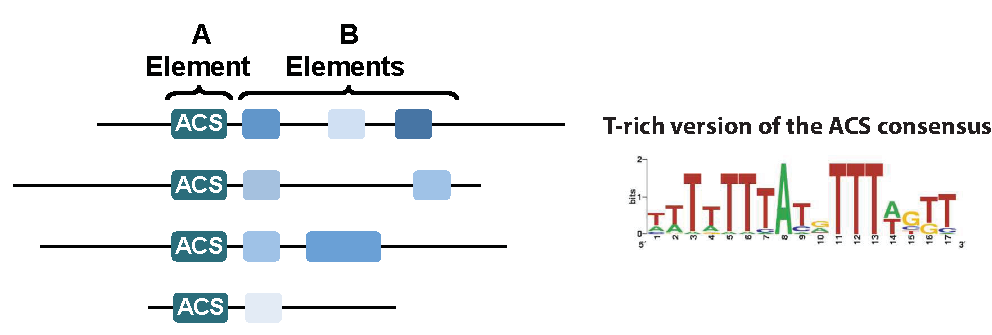
\includegraphics[width=\textwidth]{figures/results/acs}
\caption[ACS consensus an arrangement relative to other origin DNA elements]{Cartoon showing the most typical arrangement of sequence elements within origins. the ACS is required, while several B elements contribute to origin specification dowstream of the T-rich strand of the ACS.}
\label{fig:originSchema}

\end{figure}

The ACS is an AT-rich sequence element that is bound by the ORC complex and acts as the assembly site for the pre-replication complex. Because of its non-palindromic sequence, we could appropriately distinguish between transcription along the T-rich or A-rich versions of the ACS consensus. Additionally, the orientation of the ACS determines the location of other important sequence elements of the origin, the B elements (fig \ref{fig:originSchema}). This allowed us to not only be strand-specific with respect to the ACS, but with respect to the whole structure of the origin. 

\section{Transcriptional pausing and termination are associated with replication origins}

The meta-site analysis of RNAPII occupancy around replication origins is shown in fig \ref{fig:metagenes}A. The top part of the plot represents transcription along the T-rich strand of the ACS, while the bottom part represents transcription along the A-rich strand of the ACS. To obtain this plot, we used a set of origins for which the ACS was annotated \cite{nieduszynski:2006:genomewide}. Because transcription in origins is generally low, we restricted our analysis to those surrounded by convergent or tandem genes in order to have a more distinct signal. 



We detect an increase in polymerase occupancy, relative to the incoming average, in the vicinity of the ACS for both along the T- and A-rich strands of the ACS.
However, while transcription on the T-rich strand shows a distinct occupancy peak about 20-30 nucleotides before the ACS, transcription on the A-rich strand displays multiple peaks that reside 110-130 nucleotides away from it.
 Additionally, both occupancy increases—especially the one of the T-rich strand—are characterized by a steep drop in signal after their peak. Because of this sharp drop, we reasoned that the peaks could represent polymerase pausing caused by transcription termination. 
We therefore generated an aggregate plot across all origins, showing the location of termination events (as defined by the production of RNA 3’-ends \cite{wilkening:2013:efficient}) relative to the position of the ACS (fig \ref{fig:metagenes}B). 
We detected a substantial number of termination events in the vicinity of the ACS. 
Moreover, the asymmetry that we highlighted between the two strands with respect to polymerase occupancy is maintained in this analysis. 
The peak of termination events in the T-rich strand resides about 20 nucleotides from the ACS, while in the A-rich strand this peak is shifted ~100 nucleotides away from the ACS. 
These results show that RNAPII accumulates around replication origins, and this accumulation coincides with transcription termination events. 
  
\begin{figure}[hp]

\centering
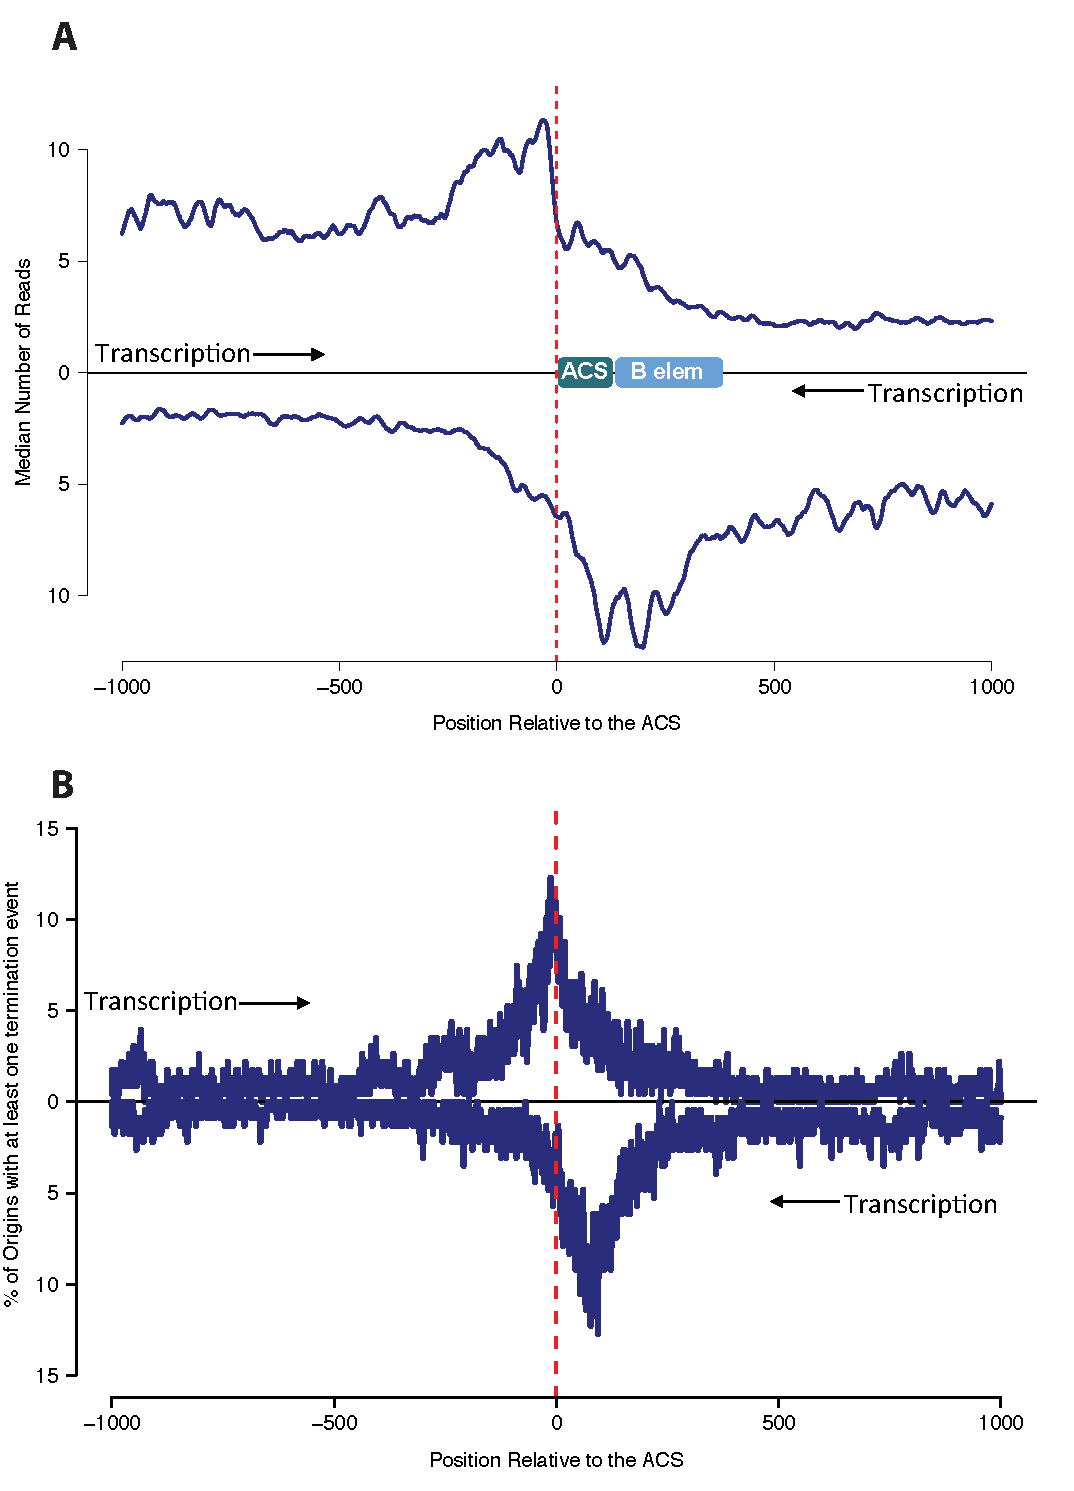
\includegraphics[width=\textwidth]{figures/results/metagenes}
\caption[Metagene analyses showing polymerase occupancy and termination around replication origins]{\textbf{A: }Metagene analysis performed on a polymerase occupancy dataset \cite{schaughency:2014:genomewide}. profiles represent the average levels of transcription across origins surrounded by convergent and tandem genes. The top part of the plot represents transcription along the T-rich strand of the ACS, while the bottom part represents transcription along the A-rich strand of the acs. \textbf{B: } Plot representing the percentage of assayed origins with at least one termination event at any given position. }
\label{fig:metagenes}

\end{figure}  
  
Although we did not know which pathway was responsible for the termination events we detected around origins, we identified several hallmarks of road-block termination. Polymerase pausing is coincident with precise termination and, at least in the case of the T-rich strand, is positioned ~20 nucleotides before the binding site of a DNA binding factor. This led us to speculate that termination in the  strand is caused by a road-block dependent on ORC. 

\begin{figure}[h]

\centering
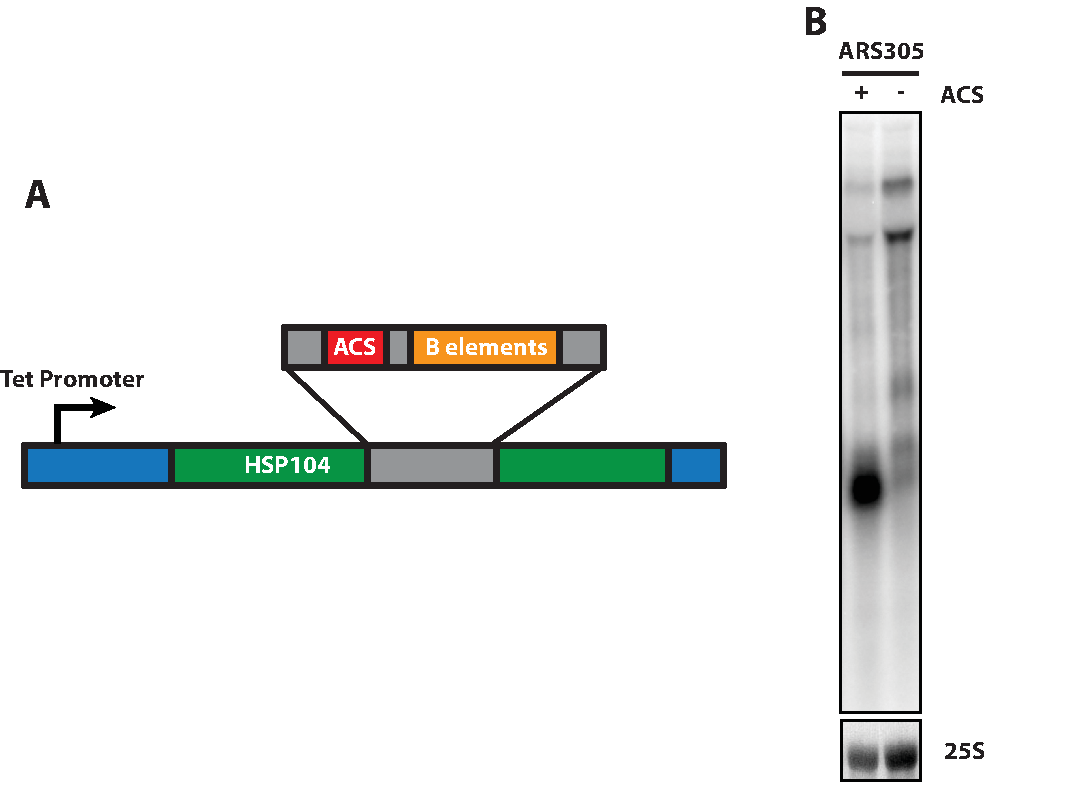
\includegraphics[width=\textwidth]{figures/results/northern}
\caption[Northern blot analysis of transcription through ARS305]{\textbf{A: }In our reporter system, a tet promoter directs transcription of a fragment of the HSP104 gene, whithin which ARS305 is embedded with or without the ACS. \textbf{B: } Northern blot analysis of the reporter system shows the presence of a short transcript that disappear upon ACS deletion. }
\label{fig:northern}

\end{figure}  

In order to test this hypothesis, Julien Gros, post-doc in the lab, performed northern blots using a reporter system. In this system, the sequence of interest is embedded in a fragment of the HSP104 gene, whose expression is then driven by a strong promoter (Fig \ref{fig:northern}A). 
We tested the sequence of origin ARS305 carrying the deletion of the ACS sequence. 
Figure \ref{fig:northern}B shows species generated by transcription through the T-rich strand of the ACS in presence or absence of the ACS sequence itself. 
Strong signal for a short transcript is detectable when the ACS is present, while in its absence, the short transcript disappears to the profit of a longer species. 
Although we cannot formally exclude that sequence elements are playing a role in transcription termination of the short species, this results argues in favor of termination by a road-block mechanism.

\section{transcription levels asymmetrically affect origin efficiency}

Road-block is known to act as fail-safe termination to protect promoter regions and other loci from transcriptional interference \cite{colin:2014:roadblock}. 
We reasoned that termination enacted by ORC could have a similar role by protecting the B elements, which are known to aid in pre-RC assembly \cite{wilmes:2002:b2}. 
Because of the arrangement of ACS and B elements within origins, however, ORC would only be able to block upstream transcription before the B elements are invaded. To test this hypothesis, we therefore correlated several measures of origin efficiency with levels of transcription upstream of the ACS on both its T-rich and A-rich strands. In order to obtain these values, we calculated the average polymerase occupancy in a 100 nucleotide window upstream of the ACS. Transcription levels calculated along the T-rich strand of the ACS were dubbed ``sense", while transcription levels calculated over the A-rich strand of the ACS were dubbed ``antisense" (figure \ref{fig:senseAntisense}).

\begin{figure}[h]

\centering
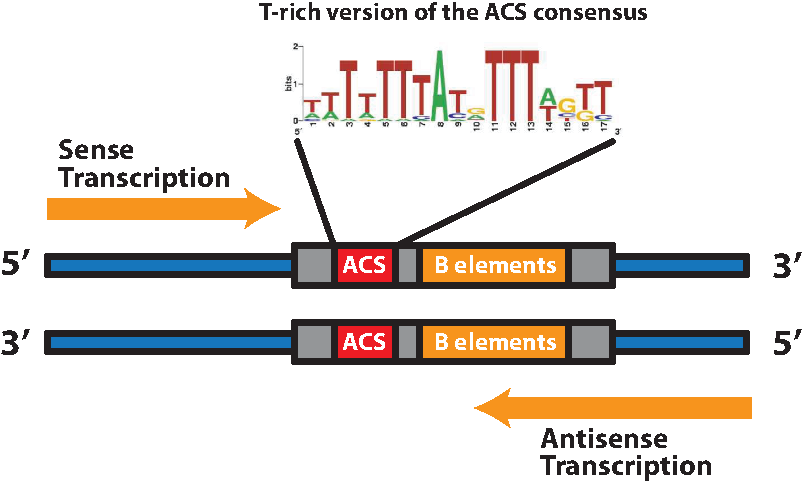
\includegraphics[width=\textwidth]{figures/results/senseAntisenseSchema}
\caption[Cartoon of sense and antisense transcription relative to the ACS]{Schematic representation of ``sense" and ``antisense" transcription relative to the structure of the origin. While sense transcription can be blocked by ORC before reaching the B elements, antisense transcription has no such impairments.}
\label{fig:senseAntisense}

\end{figure}  

As replication occurs in discrete steps, we wanted to know if either sense or antisense transcription were affecting any particular stage of replication initiation. We therefore correlated per-origin estimates of licensing efficiency, firing efficiency, and timing of firing (niedu) with our estimates of sense and antisense transcription. Our approach was two-fold: for every measure of origin efficiency, we calculated the Pearson’s correlation between it and the levels of sense and antisense transcription. In parallel, we obtained two subpopulations of origins, according to either transcription or efficiency, and compared them using boxplots and t-tests for statistical significance.

\subsection{Licensing efficiency}

Licensing is the first step in DNA replication, however, not all origins are licensed during the cell cycle.
Every origin we considered is associated with a value between zero and one, representing the likelihood that the origin will be licensed during the cell cycle \cite{hawkins:2013:highresolution}. 
We split the population of origins into two sub-populations according to high and low transcription for both sense and antisense. 
We then compared the distribution of licensing efficiencies in these two sub-populations. 
Analysis of the overall populations showed no difference in licencing efficiency whether origins are surrounded by high or low sense or antisense transcription (fig \ref{fig:licensing}A). 
A statistically significant anti-correlation between antisense transcription levels and licensing efficiency (pearson’s $\rho$ = -0.15 with $p$ = 0.03) could be observed, but no significant correlation between sense transcription levels and licensing efficiency (pearson’s $\rho$ = -0.04 with $p$ = 0.53). 
We reasoned that the low levels of endogenous transcription might not be sufficient to affect highly efficient origins. We therefore considered only origins with relatively low licensing efficiency ($<$ 0.6) and repeated the experiment (fig \ref{fig:licensing}B).
\begin{figure}[hp!]

\centering
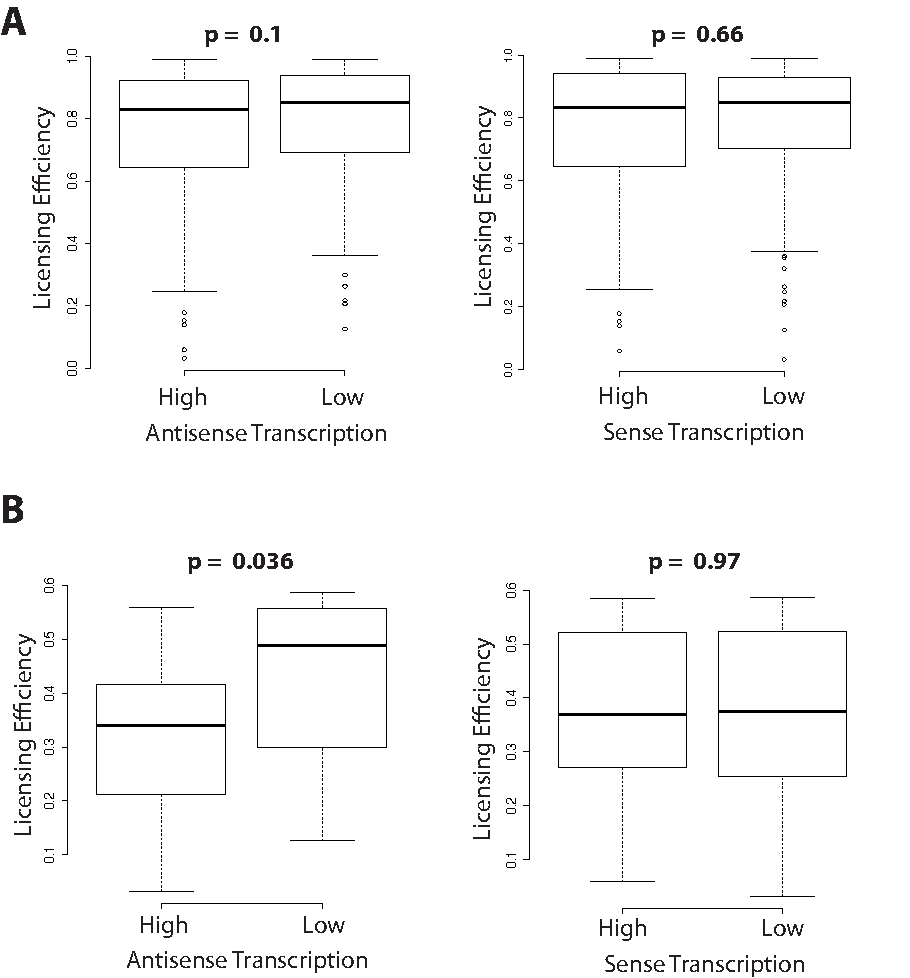
\includegraphics[width=\textwidth]{figures/results/competence}
\caption[boxplots comparing licensing efficiencies in high- and low-transcription populations]{These boxplots compare the distribution of licensing efficiencies between high- and low-transcription populations.\textbf{A: }Boxplots generated using the totality of the origins available to us. high- and low-transcription populations show similar levels of efficiency both according to sense and antisense transcription. \textbf{B: } In this experiment, we restricted our boxplots to poorly licensed origins. Higher levels of antisense transcription are now significantly associated with lower efficiency, while high or low sense transcription displays no difference. }
\label{fig:licensing}

\end{figure}  
A significant difference in the distribution of licensing efficiencies could be detected between populations with high and low antisense transcription. 
However, no such a difference could be detected when the two populations were chosen according to sense transcription. 
These results are supported by the Pearson’s correlation coefficients: the anti-correlation between antisense transcription and licensing efficiency is higher (pearson’s $\rho$ = -0.32 with $p$ = 0.04), while that between sense transcription and licensing efficiency remains low (pearson’s $\rho$ = 0.03 with $p$ = 0.83). 
Taken together, these results support the notion that physiological levels of transcription antisense to the ACS can negatively affect licensing origins, while sense transcription—regardless of its intensity—does not affect significantly licensing efficiency.



\subsection{Firing efficiency}

Firing is the process that allows licensed origins to activate and begin the replicative process. This step is conditional on the presence of the pre-replication complex, and therefore cannot occur unless the origin has been previously licensed. To define classes of origins with different firing efficiencies, we compared licensing and firing for every origin using published data. As for licencing, the probability of firing has been defined by a value between 0 and 1 \cite{hawkins:2013:highresolution}.

A scatterplot of firing and licensing efficiencies is represented in fig \ref{fig:firing}A. We divided origins into two populations according to their position in this plot. Origins residing around the diagonal are able to fire efficiently, as licensing and firing have similar likelihoods and firing requires licensing. Origins residing below the diagonal, however, fire inefficiently, as their firing efficiency is lower than their licensing efficiency. in fig \ref{fig:firing}B we compare the distribution of antisense and sense transcription levels between these two populations. Inefficiently firing origins display higher levels of antisense transcription relative to efficiently firing origins, however, this relationship is lost when considering sense transcription. These results are supported by Pearson’s correlations: antisense transcription is anti-correlated with normalized firing efficiencies (pearson’s $\rho$ = -0.18 with $p$ = 0.01) while sense transcription and normalized firing efficiencies do not seem to be correlated at all (pearson’s $\rho$ = 0.06 with $p$ = 0.39). taken together, these results suggest that not only licensing, but also firing is affected by antisense transcription levels, while sense transcription levels have no effect on this step.
\begin{figure}[h!]

\centering
\includegraphics[width=\textwidth]{figures/results/firing}
\caption[boxplots comparing transcription levels in high- and low-firing populations]{These boxplots compare the distribution of sense an antisense transcription levels between populations with high and low firing efficiency. \textbf{A: }Plot of licensing efficiency vs firing efficiency. Because firing requires licensing, similar efficiency values in these two metrics denote highly efficiently firing origins. We therefore consider those origins close to the diagonal as efficient origins and those below as inefficient. \textbf{B: } Boxplots comparing the distribution of sense and antisense transcription levels between origins with low and high firing efficiency. The population with low firing efficiency are significantly associated with higher antisense transcription levels, but this relationship does not hold in the case of sense transcription. }
\label{fig:firing}

\end{figure} 

\subsection{Timing of firing}

While firing efficiency is a measure of how often a particular origin is able to initiate DNA replication, it does not give information about the elapsed time between the entry in S-phase and activation of the replisome (time of firing). We wanted to assess whether transcription levels influence the timing of origin firing. In fig \ref{fig:timing} we compare the distribution of median firing times for high and low, sense and antisense transcription. High antisense transcription is significantly associated with higher median replication times, while no difference in median replication times can be detected between high or low sense transcription levels. These results are also supported by correlations that do not rely on subpopulations: antisense transcription levels positively correlate with median replication times (pearson’s $\rho$ = 0.19 with $p$ = 0.008) while sense transcription levels show no correlation (pearson’s $\rho$ = -0.05 with $p$ = 0.42). These results suggest that even when firing occurs, antisense transcription levels can delay firing, possibly by interfering with the assembly of the replisome, while sense transcription levels have no impact.
\begin{figure}[h!]

\centering
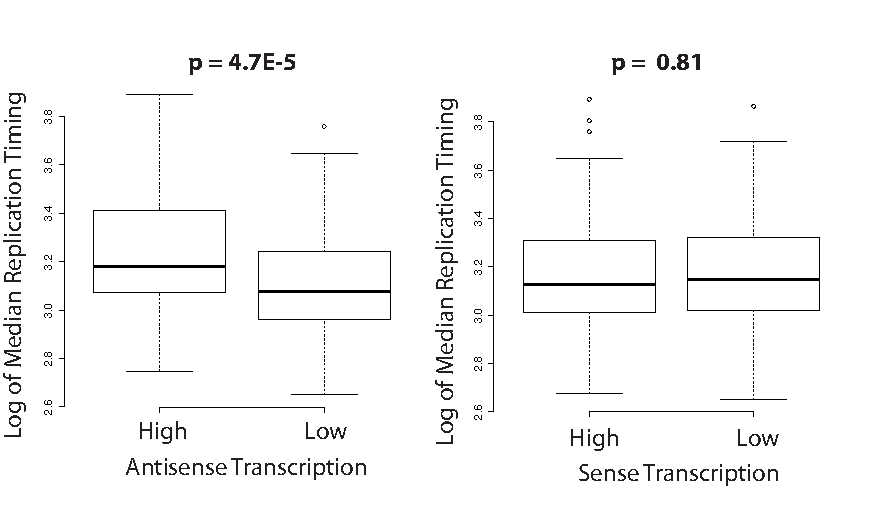
\includegraphics[width=0.97\textwidth]{figures/results/timing}
\caption[boxplots comparing median replication times in high- and low-transcription populations]{These boxplots represent the distribution of median replication times in population with high, low, sense, and antisense transcription. High antisense transcription correlates with higher replication times relative to low antisense transcription. However, sense high and low sense transcription seems to have no effect on replication timing.}
\label{fig:timing}

\end{figure} 


\section{Discussion}

In this work, we investigated the relationship between the process of origin specification and that of RNA transcription. We analyzed transcription around replication origins separately on both strands and detected localized increases in polymerase occupancy that coincided with hotspots of transcription termination. We noticed that pausing and termination were arranged asymmetrically relatively to the ACS, with a major peak immediately upstream of the ACS in the T-rich orientation (position -25) of and several peaks indicating accumulation of polymerases at different distances (-100 to -125) upstream of the ACS in the  A-rich  orientation.

We explored the possibility that ORC binding to the ACS might induce road-block termination at these sites through northern blot analysis of ARS305. This experiment revealed that transcription upstream of the ACS in the T-rich strand orientation is terminated in an ACS-dependent manner. Experiments were also performed to assess the occurrence of termination for transcription entering the ACS from the opposite direction (upstream of the A-rich strand) but the results were not conclusive because a site of NNS-dependent termination was present that masked the possible ACS-dependent termination. At this stage we do not know whether the additional peaks of polymerase pausing at position -100 to -125 upstream of the ACS in the A-rich strand orientation are due to roadblocked polymerases or polymerases paused for other reasons.  

However, prompted by the asymmetry revealed by these experiments, we tested the hypothesis that transcription levels could asymmetrically impact origin efficiency depending on origin orientation. We correlated per-origin estimates of licensing efficiency, firing efficiency, and timing of firing with surrounding transcription levels both sense and antisense relative to origins oriented by the T-rich strand of the ACS. High levels of transcription on the antisense strand proved to negatively impact every measure of replication efficiency, while sense transcription had no significant effect.

\subsection{Transcription termination is a feature of replication origins}

Our meta-site analyses provided insights on the global state of polymerase occupancy and transcription termination around replication origins genome-wide. According to this global view, many origins are associated with distinct peaks of polymerase pausing and transcription termination on both sense and antisense strands. Because of the complexity of the DNA replication process, as well as previous evidence emerging from the literature, we speculate that these termination events protect the origin by preventing transcriptional interference. In accordance with this model, we have evidence that transcription on the sense strand of the ACS is terminated by ORC through road-block, a mechanism already known to protect promoter regions from invading polymerases. This model is supported by preliminary analyses of polymerase occupancy datasets generated in strains defective for either CPF or NNS termination. Both datasets displayed a marked increase in polymerase pausing in the vicinity of ORC, a phenotype consistent with the increased readthrough transcription that is stalled at the site of road-block. While the meta-site analyses provided many elements that suggested road-block by ORC, we could not formally prove that its presence is responsible for the termination. In our case study, ARS305, we show that termination is ACS dependent, but cannot exclude that sequence elements within the ACS could be the determinant for termination. 

\subsection{ACS orientation determines the impact of transcription on replication efficiency}

In order to explore the impact of endogenous transcription on DNA replication, we decided to correlate strand specific transcription levels with measures of origin efficiency. Through these analyses we showed that high levels of transcription generally correlate with poor replication performance, however, only transcription entering the origin from upstream of the A-rich strand of the ACS displays such correlations. We propose a model whereby a road-block enacted by ORC is sufficient to prevent endogenous levels of RNAPII from elongating into the B elements, thus preventing transcription from interfering with the replicative process (fig \ref{fig:model}). Transcription on the other strand, however, might be terminated less efficiently which might not be sufficient to prevent all incoming polymerases from invading the B elements and affecting one or more DNA replication steps. 

\begin{figure}[h]

\centering
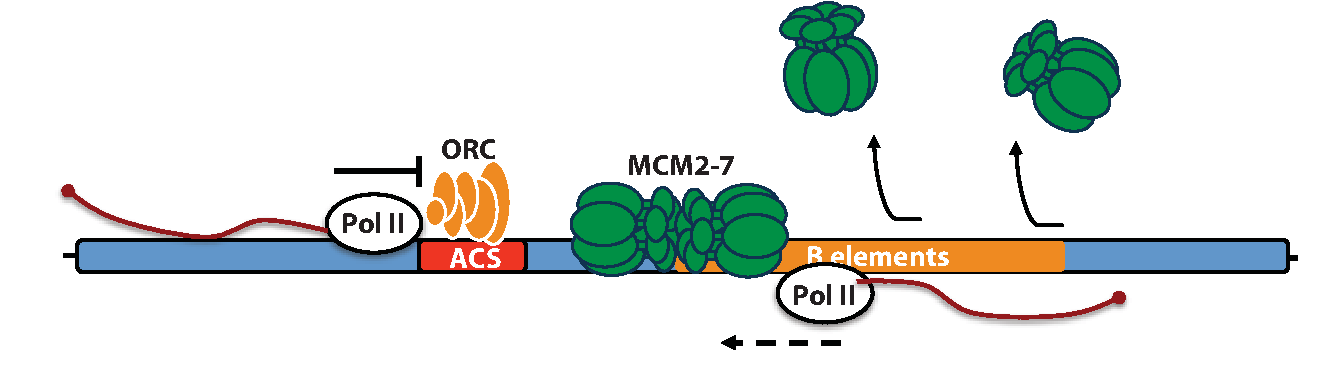
\includegraphics[width=\textwidth]{figures/results/model}
\caption[A model of how transcription can affect replication efficiency]{Model of how transcription can asymmetrically affect replication efficiency. While sense transcription can be efficiently blocked by the ACS before reaching the B elements, antisense transcription can invade the B elements more efficiently.}
\label{fig:model}

\end{figure} 

Julien Soudet, one of our collaborators, generated some preliminary data measuring replication efficiency in a strain defective for NNS termination. We calculated Pearson’s correlation between antisense transcription levels and replicative efficiency relative to wild type. A strong anticorrelation between the two quantities was observed (figure \ref{fig:JS}), implying that stronger antisense transcription relative to wild type is associated with reduced replication activity. Surprisingly, correlation between relative sense transcription levels and relative replicative efficiency also displays a negative trend (figure \ref{fig:JS}), albeit lower than in the antisense case. These results suggest that the increased transcription resulting from defects in NNS termination are enough to overcome the road-block and generate defects in replication efficiency independent of the orientation of the origin. however, they also suggest that transcription termination on the sense strand is likely stronger than that on the antisense strand, as it is less associated with poor replicative performance. 

\begin{figure}[h]

\centering
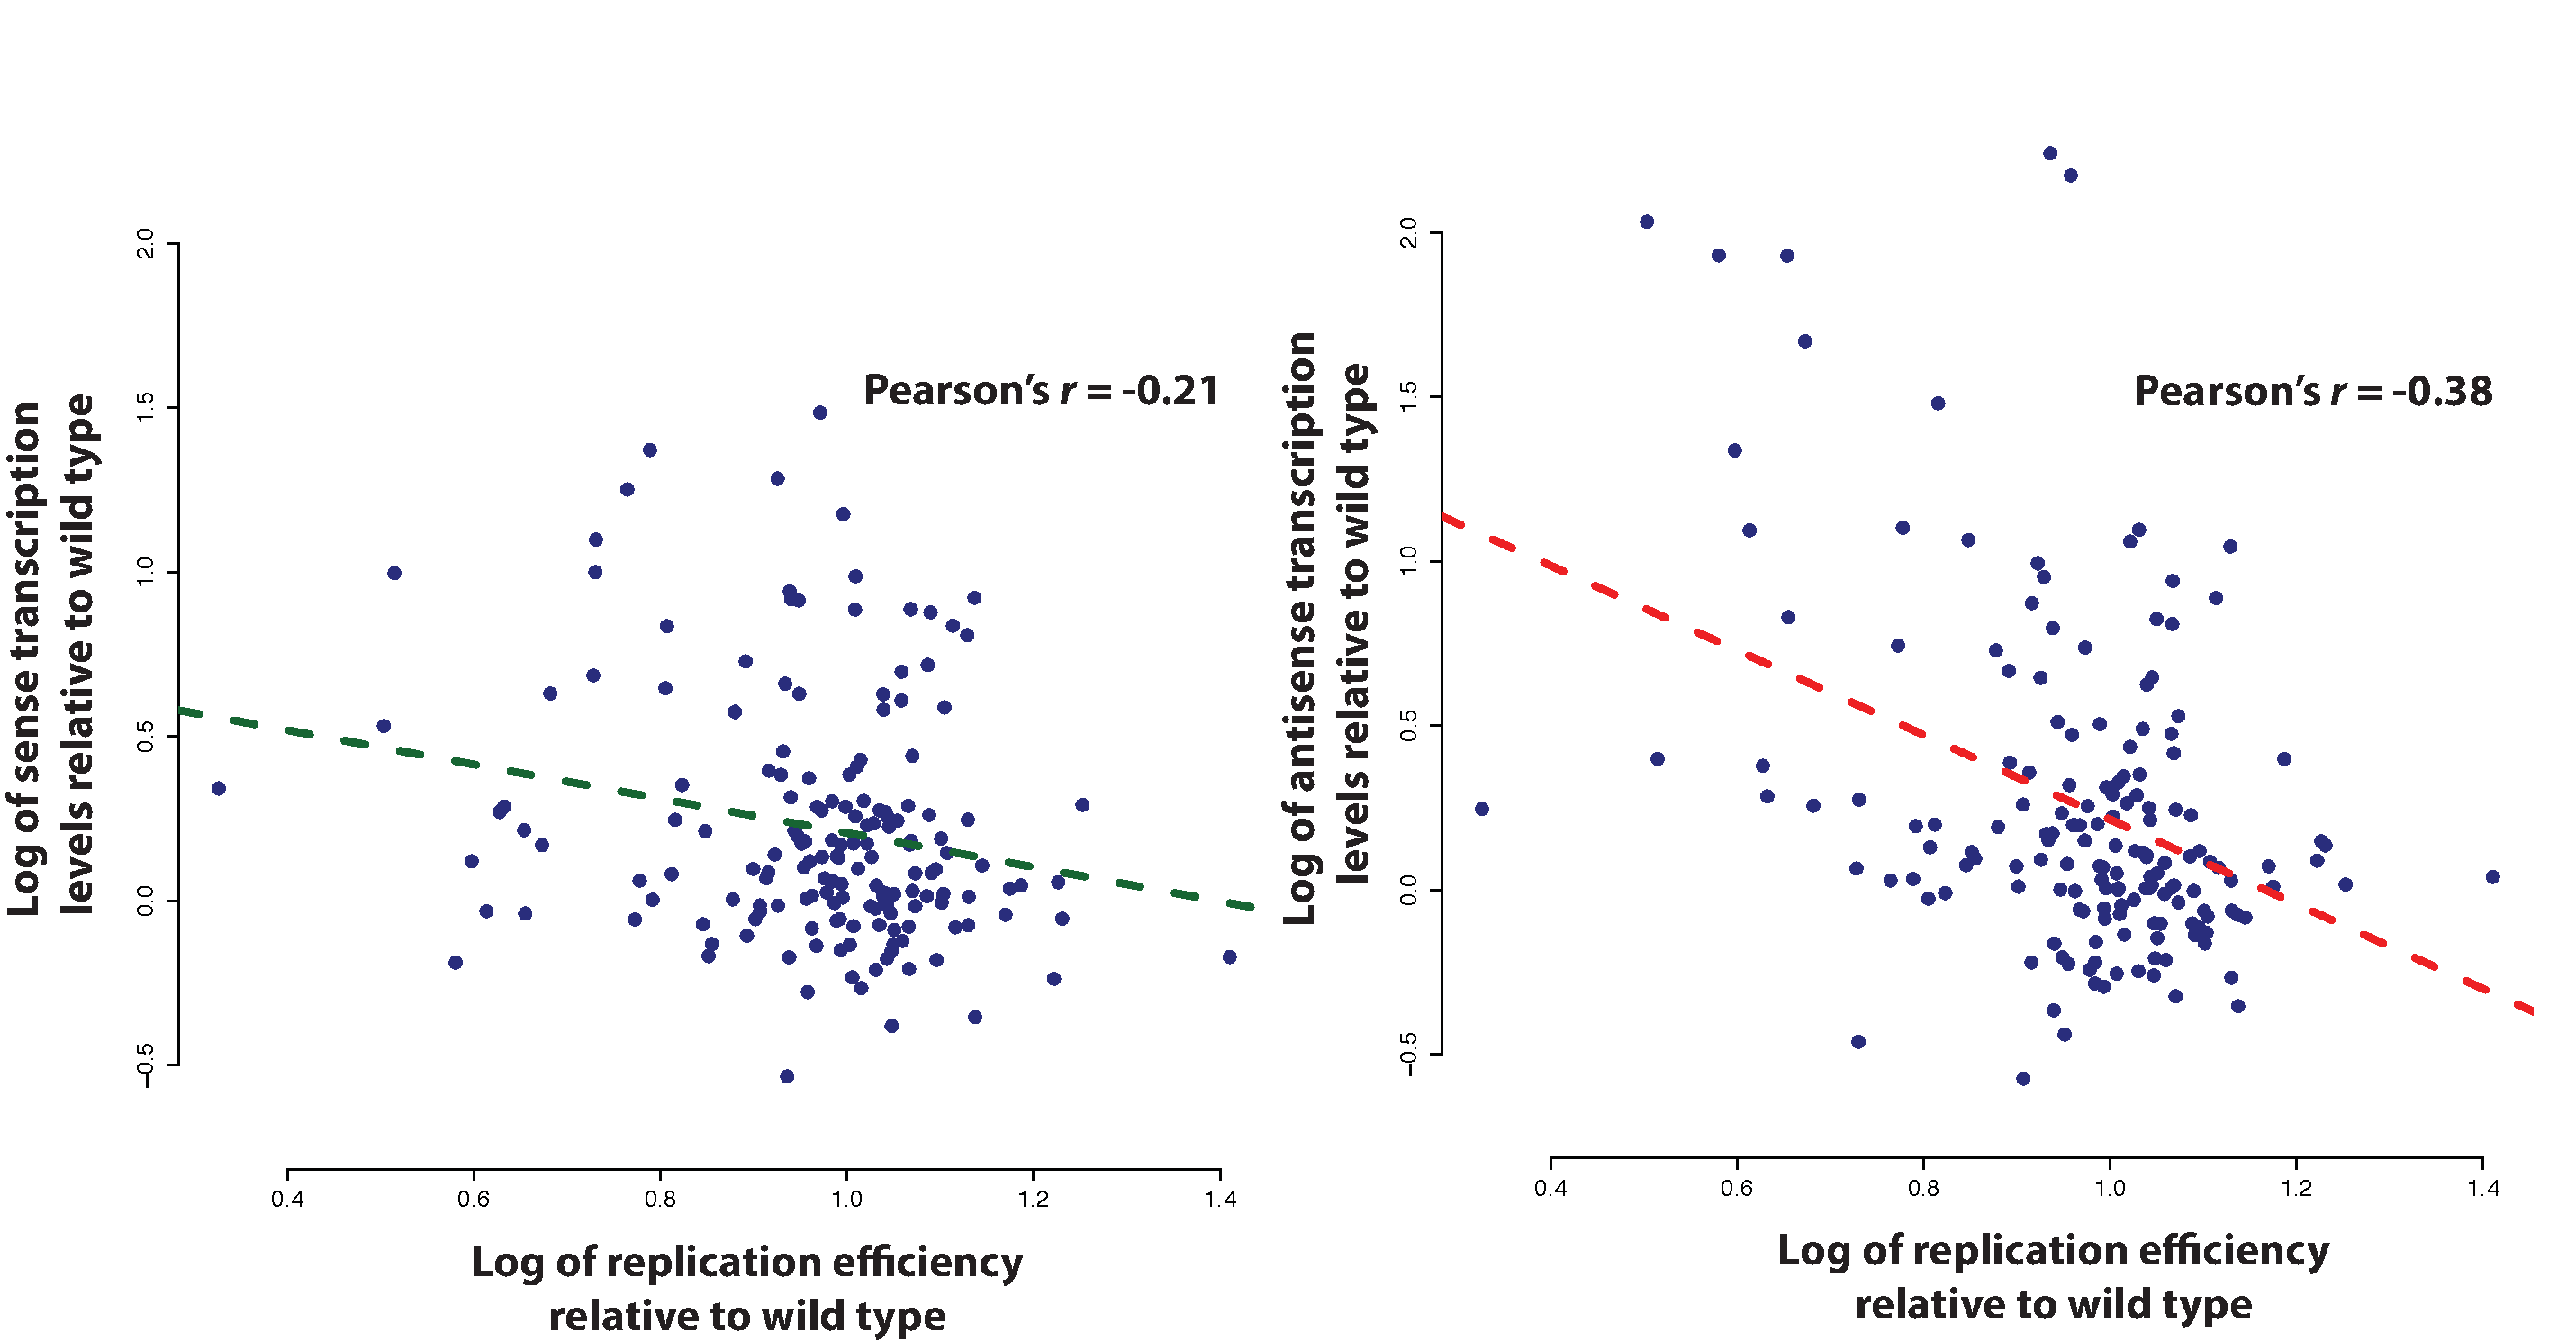
\includegraphics[width=\textwidth]{figures/results/JScorrelations}
\caption[correlations between transcription and replication efficiency in a NNS defective strain]{Scatterplots of relative sense and antisense transcription levels versus relative replication efficiencies. Each axis displays the log$_2$ ratio between levels of transcription or replication efficiency in a NNS-defective strain relative to wild type. In this non-physiological condition, both sense and antisense transcription levels anticorrelate with replication efficiency. However, antisense transcription levels remain more strongly associated with poor replicative efficiency.}
\label{fig:model}

\end{figure} 


Overall, downregulation of replicative activity seems to be a function of the quantity of polymerases that transcribes through the core sequence elements of the origin. However, it is difficult to assess the mechanistic reasons for this phenotype. Transcription might directly displace or otherwise interfere with elements of the pre-RC. Alternatively, it is tempting to speculate that transcription-dependent nucleosome deposition might interfere with assembly or firing of the replication complex.

%	\input{chapters/results/selex.tex}


\part{Materials and Methods}




%\backmatter
\bibliographystyle{acm}
\bibliography{references,fixed_references}
\end{document}